\chapter{Drift Chamber 05} \label{ch::dc05}
\ifpdf
\graphicspath{{Chapters/DC5/Figs/}}
\fi

Drift Chamber 05 (DC05) is a large-area planar drift chamber.  It was
constructed in 2014 and 2015 at the University of Illinois and Old Dominion
University and was then shipped to CERN for final assemble.  DC5 was installed
to the large angle spectrometer of COMPASS during the spring of 2015.

The DC5 detector is an import tracking detector, which successfully collected
data from 2015 through 2018 and will continue to be an important component for
track reconstruction in future measurements.  The author of this thesis
significantly contributed to the prototyping and construction at Illinois and
the assembly at CERN and as well for performing calibrations and maintaining
DC5.


\section{Motivation for Drift Chamber 05}

Simulations of the COMPASS spectrometer for Drell-Yan measurements determined
that 96\% of all events include a track in the large angle
spectrometer~\cite{proposal}.  For this reason the Drell-Yan trigger system was
designed only to record events with at least one track in LAS.  As DC5 was
installed in LAS it is therefore very important in track reconstruction for
Drell-Yan measurements.  In fact it was so essential to have the LAS operating
optimally that DC5 replaced an aging straw detector.  Additional
simulations with the Drell-Yan setup and this corresponding COMPASS Drell-Yan
trigger showed that the global reconstruction efficiency drops below 30\%
without DC5 and half of another large area tracker in
LAS~\cite{quintans_rec_march12}.  That is to say the spectrometer reconstruction
efficiency is very poor without DC05 and half of another LAS large area tracker
with unstable performance.  Fig.~\ref{fig::standardRec} and
Fig.~\ref{fig::withLARec} show the nominal global reconstruction efficiency and
the worst case scenario for Drell-Yan measurements respectively.  For these
reasons it was very important to have DC05 installed and working reliably.

\begin{figure}[h!t]
  \centering
  \begin{subfigure}{.5\textwidth}
    \centering 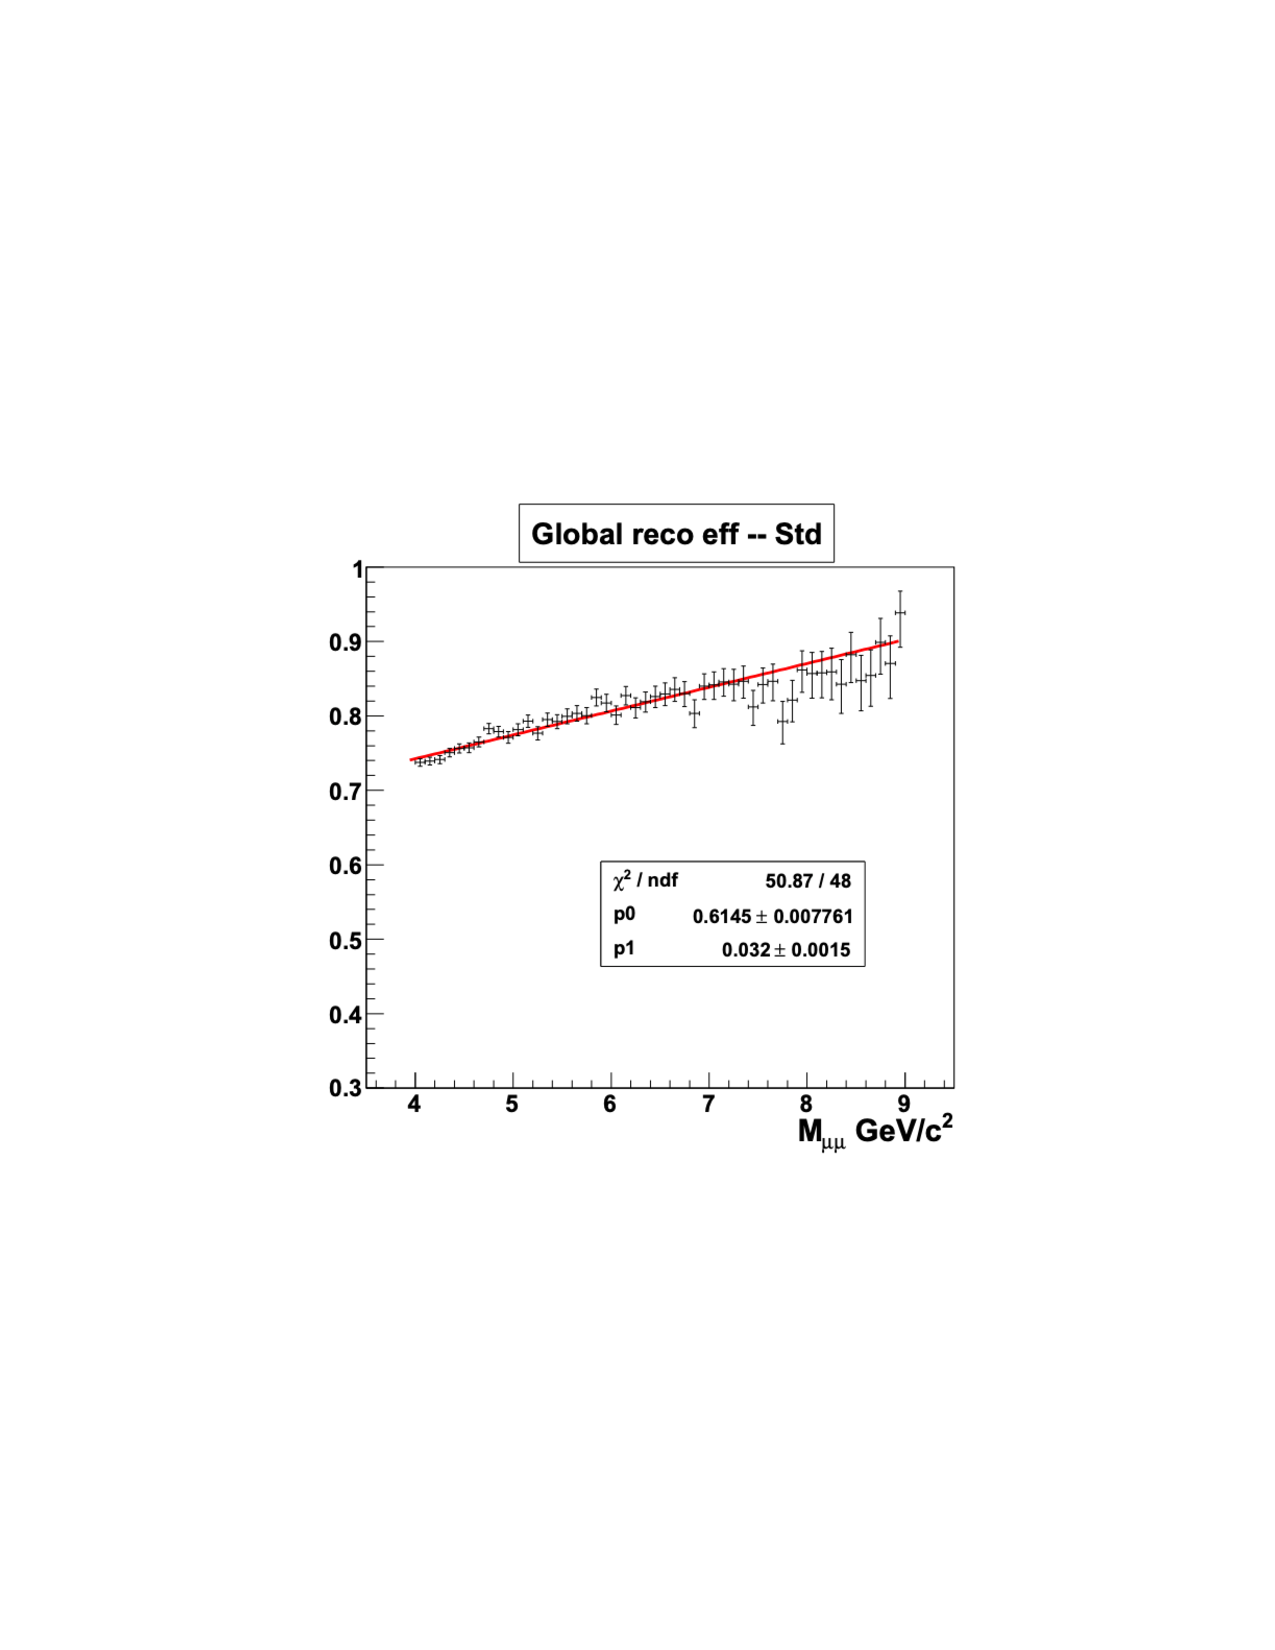
\includegraphics[width=\linewidth, trim=5cm 8cm 5cm 8cm,
      clip]{standardRec}
    \caption{Global reconstruction efficiency with all detectors working.  This
      image was taken from~\cite{quintans_rec_march28}}
    \label{fig::standardRec}
  \end{subfigure}%
  \begin{subfigure}{.5\textwidth}
    \centering
    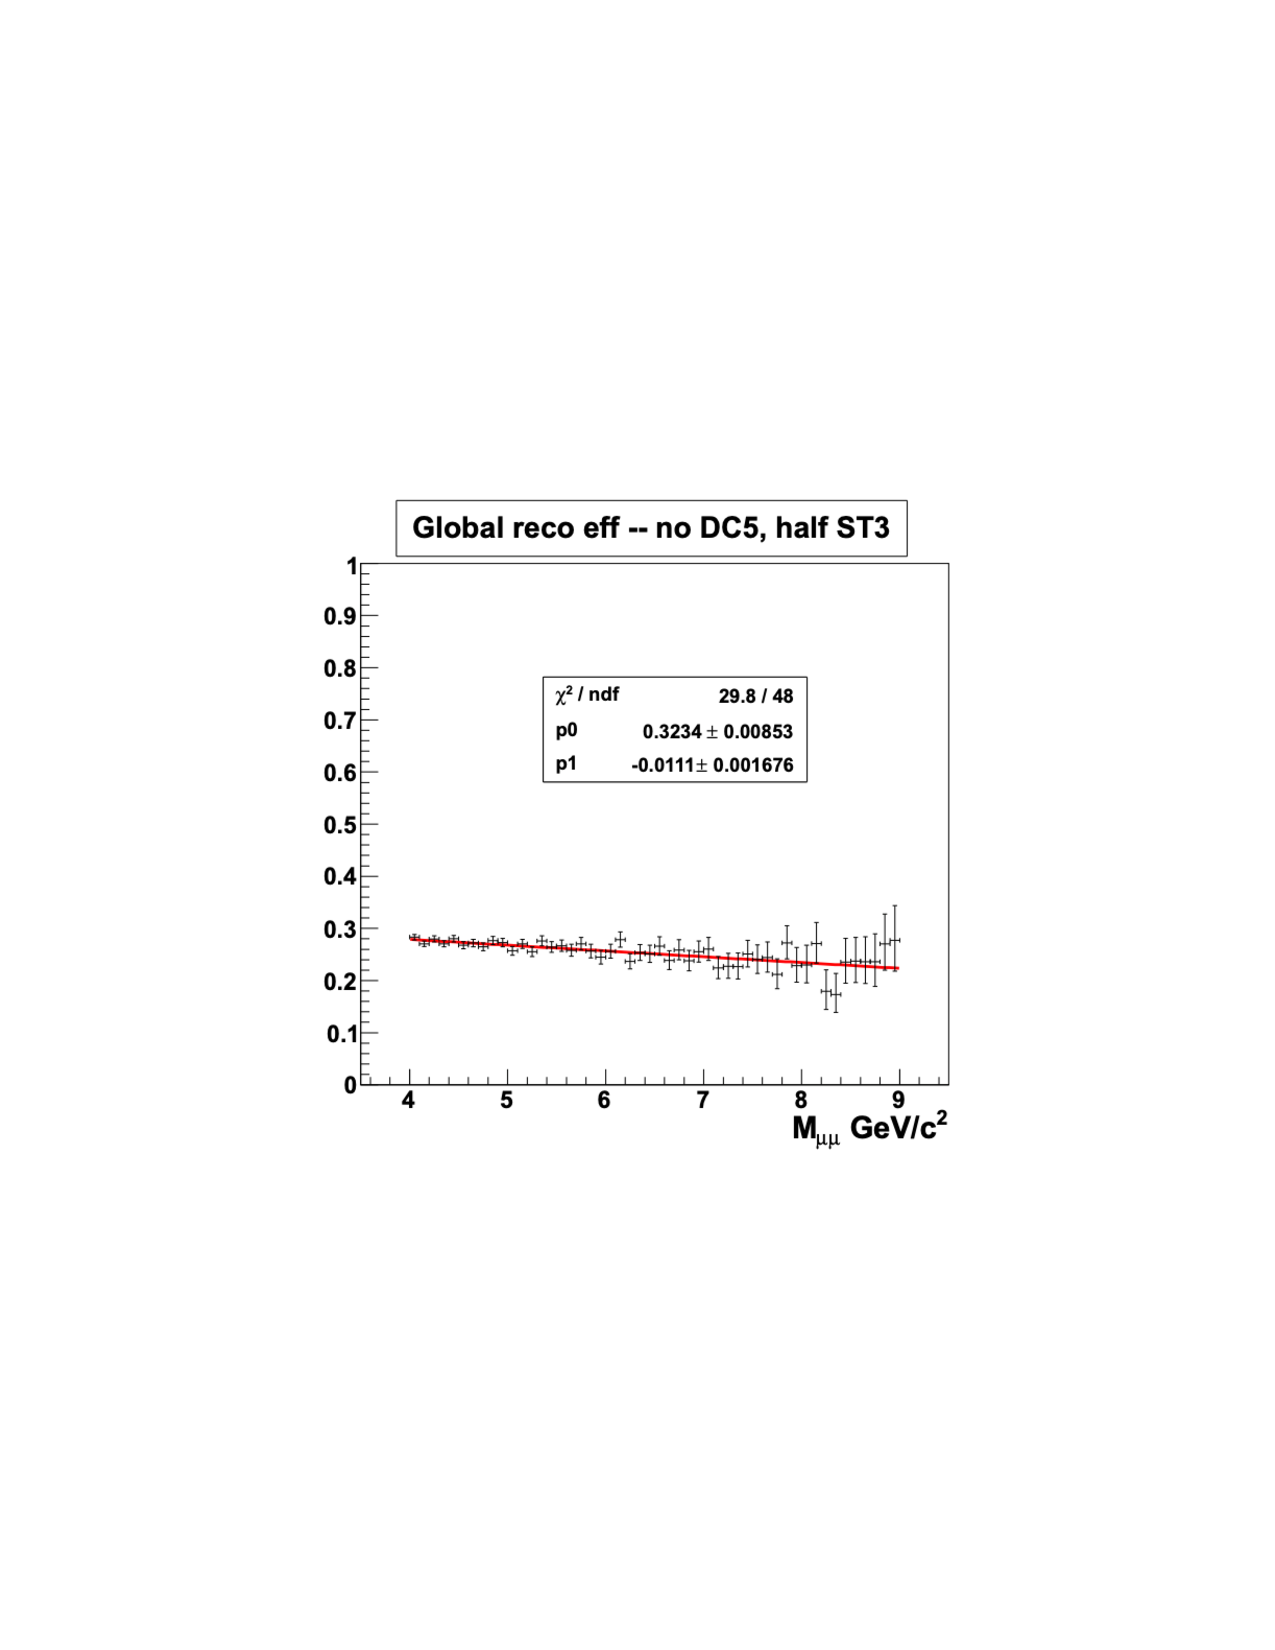
\includegraphics[width=\linewidth, trim=5cm 8cm 5cm 7.5cm, clip]{withLARec}
    \caption{Global reconstruction efficiency without DC05 and half of another
      LAS large area tracker.  This image was taken
      from~\cite{quintans_rec_march28}}
    \label{fig::withLARec}
  \end{subfigure}
\end{figure}


\section{Operating Principle}

Drift chambers are tracking detectors which can detect the location of a high
energy charge particle passing through them.  A drift chamber is built up of an
array of drift cells where at the center of each drift cell is an anode signal
wire (also called a sense wire).  Surrounding the signal wire are cathodes which
close off the drift cell.  The cathodes are set at a higher high voltage than
the anode and therefore there is an electric potential difference between the
cathode to the anode.  Fig.~\ref{fig::dcCellFieldLines} shows an example of a
drift chamber cell and the equipotential lines within the cell.  In DC05 there
are two cathode planes on top and bottom of the drift cell and a cathode field
wire adjacent to either side of the sense wire as in
Fig.~\ref{fig::DCoperation}.

\begin{figure}[h!t]
  \centering
  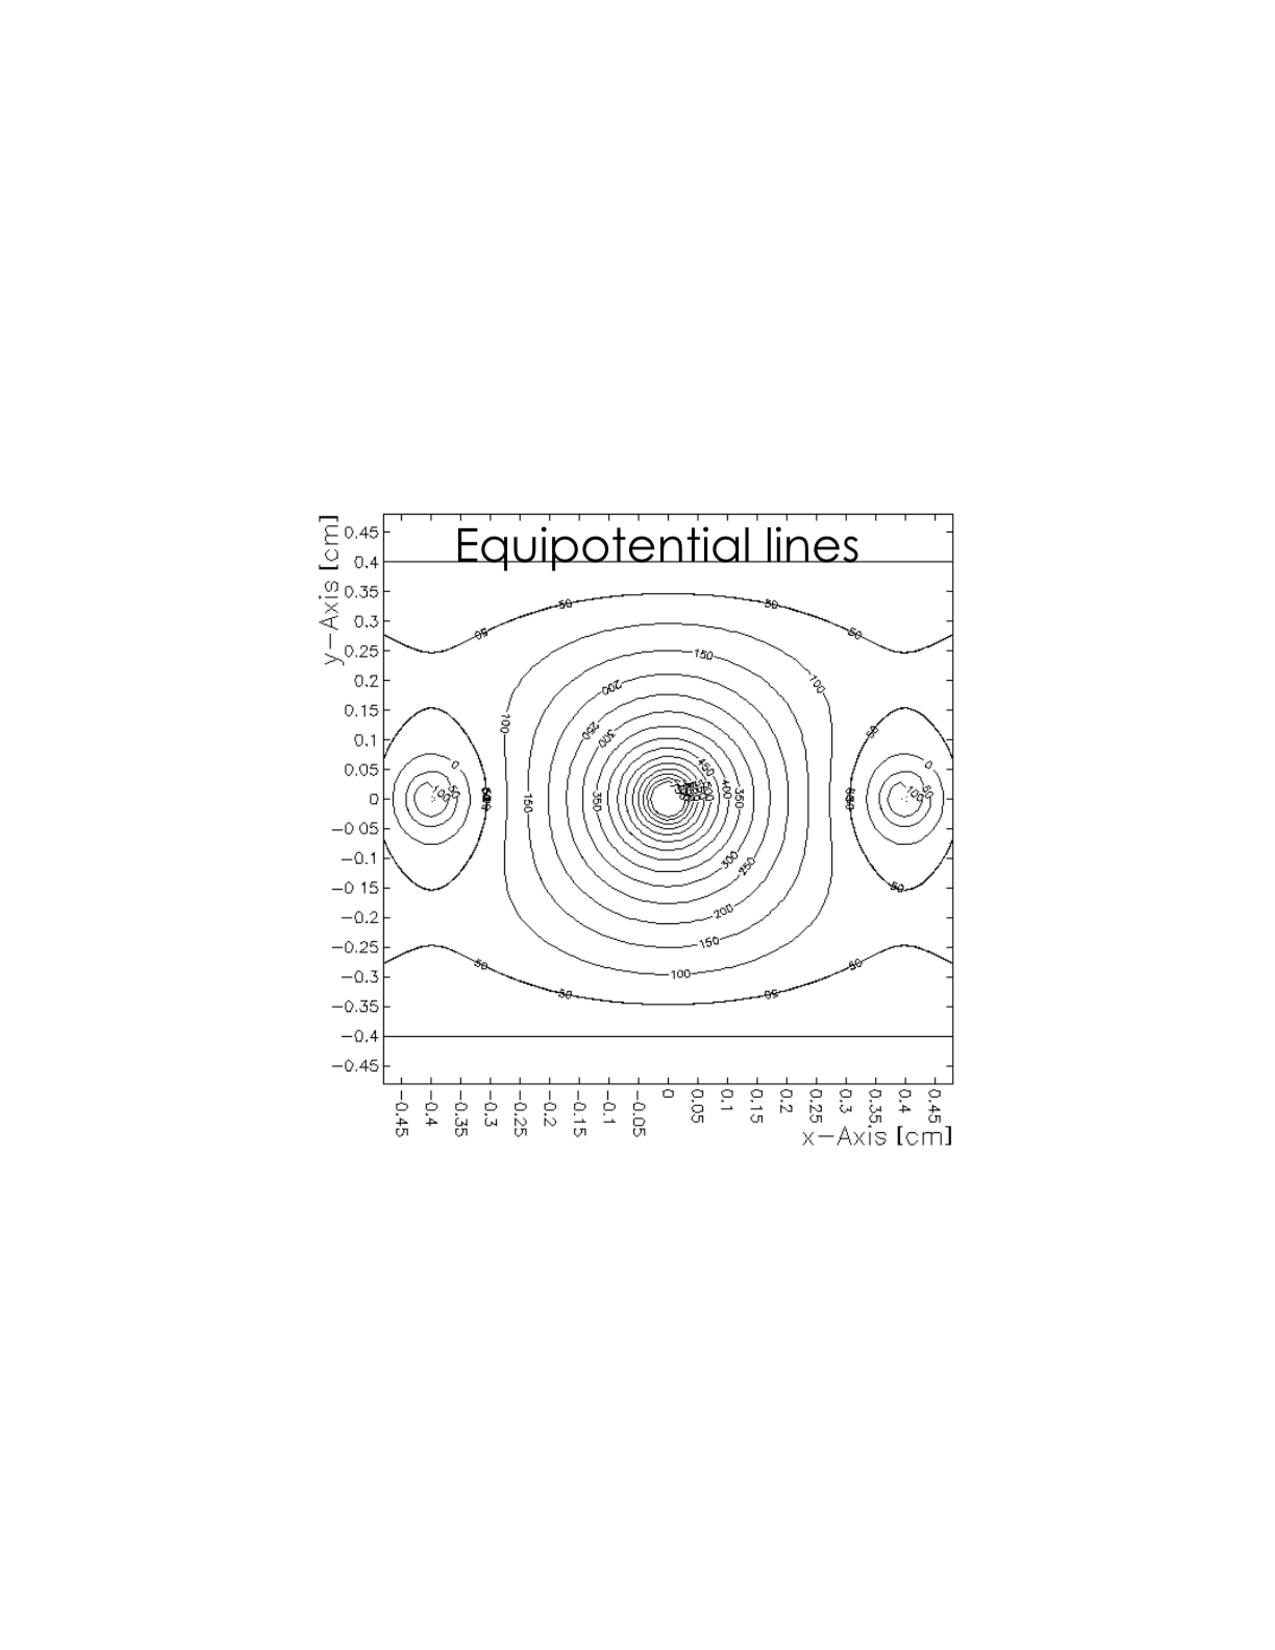
\includegraphics[width=0.6\textwidth, trim=4.5cm 8cm 4.5cm 8cm, clip]
                  {dcCellFieldLines}
  \caption{View down the axis of a drift cell and the equal voltages for this
    drift cell configuration.  This image is taken from~\cite{ran_bi}}
  \label{fig::dcCellFieldLines}
\end{figure}

Between the anodes and cathodes of a drift cell is a gas mixture.  The high
energy charged particles which enter the chamber ionize this gas mixture.  For
each track passing through the chamber, multiple primary ionization electrons
are produced and these electrons drift to the signal wire.  The number of
primary ionization electrons produced however, is not enough to create a
detectable signal on the sense wires.  For this reason the electric field
increases as the inverse of the distance from the sense wire which allows the
primary ionization electrons to gain enough energy to further ionize the gas and
ultimately produce an electron avalanche near the sense wire.  The signal
created from this electron avalanche is strong enough to detect.  A typical
detector is built so that an avalanche can occur before the sense wire but not
before a cathode wire.  This is accomplished by constructing the chamber with
sense wires having a much smaller diameter than the field wires, meaning the
electric field near the sense wire can be much larger than the electric field
near the field wire.

An important factor for a drift chamber is that the location of the primary
ionized electrons can be determined within a drift cell.  This knowledge allows
for a better position determination of the passing track as compared to a
multi-wire proportional chamber as multi-wire proportional chambers cannot
measure an RT relation.  Each sense wire records the time a signal was detected
from a track.  For the same track, the trigger records the time the track enter
the drift chamber and therefore the difference in time between the sense wire
time and the trigger time is the drift time.  For a drift chamber it is possible
to produce a calibration curve which determines the position within a drift cell
for a given drift time.  This calibration curve is so-called the RT relation.

Even with a properly calibrated RT relation the track location is ambiguous from
only one drift cell.  This is because a single drift cell can only determine a
track location as a distance from the sense wire.  Therefore it is ambiguous
where along the sense wire the track passed and also if the track passed to the
left or right of the sense wire.  For this reason drift chambers are built with
several planes in series.  A drift cell with the same orientation but shifted
with respect to the first drift cell is used to distinguish left and right
ambiguity and another cell with an orientation at an angle with respect to the
first is used to determine where along the wire the track passed.


\section{Preparation for DC05}

One of the first steps in preparation for constructing DC05 was to simulate the
detector response using Garfield~\cite{garfield}.  The purpose of these
simulations was to determine an operating threshold capable of achieving a
200~$\mu$m position resolution.  With this position resolution goal in mind,
Garfield simulated the electric potential field in each drift cell, as shown in
Fig.~\ref{fig::dcCellFieldLines}, and was able to determine the arrival times
for ionized electrons as a function of the number of primary ionized electrons
for detection.  This is important because the timing distribution for electron
arrival times gets wider and therefore worsens the position knowledge as the
number of primary electrons required for a signal increases.  The variance of
the electron arrival times was then used to determine the position resolution as
a function of the number of primary electrons needed for detection.  As is shown
in Fig~\ref{fig::PosResVnumElec}, the threshold should be tuned to detect the
amplification of the fifth primary electron~\cite{ran_bi}.  As is shown in
Fig.~\ref{fig::currentVtimeFifthElec} based on the simulation of the integrated
induced current versus the drift arrival time, the threshold for detecting the
signal should be no greater than 4~fC~\cite{ran_bi}.  This threshold charge is
determined by multiplying the induced current by the arrival time.  The
threshold was accordingly one of the design goals for the front-end electronics.

\begin{figure}[h!t]
  \centering
  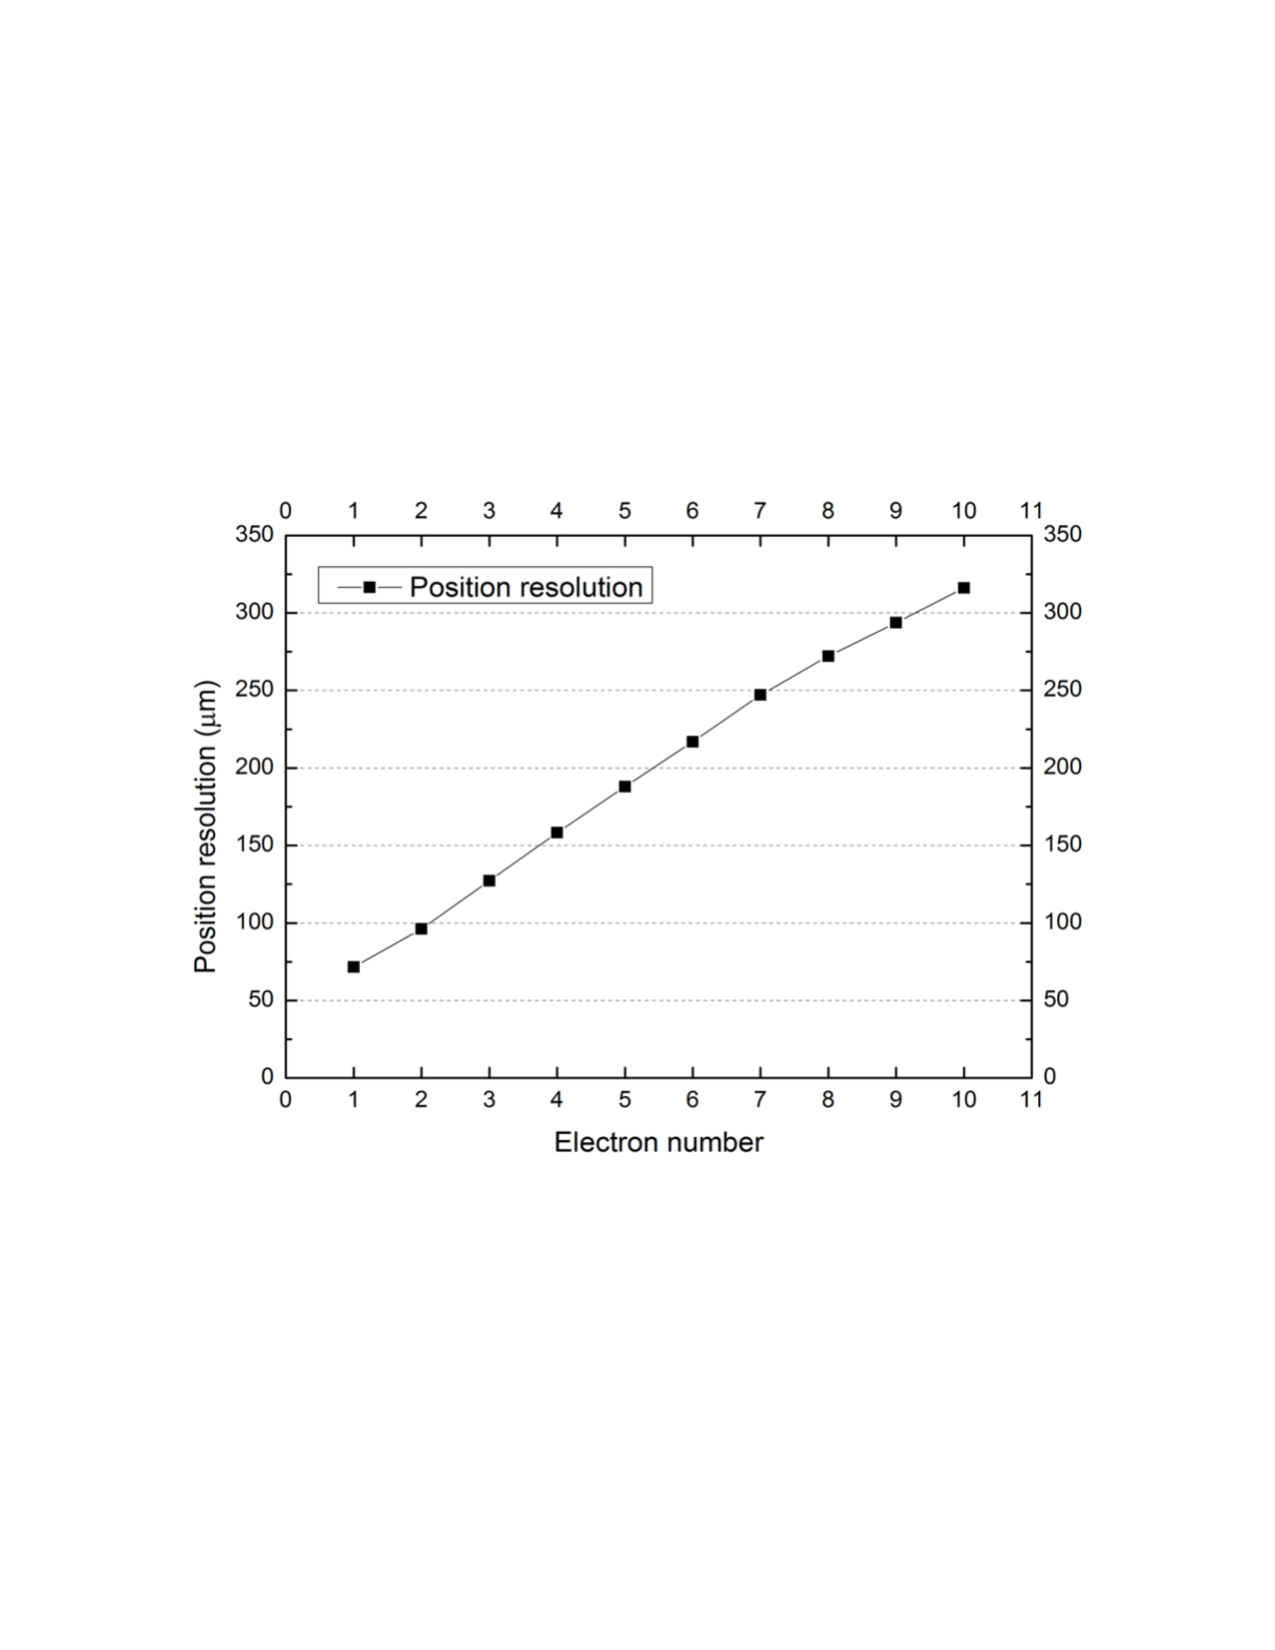
\includegraphics[width=0.55\textwidth, trim=3cm 8cm 3cm 8cm, clip]
                  {PosResVnumElec}
  \caption{A simulation of the position resolution as a function of the number
    of primary electrons needed to record a signal.  This image is taken
    from~\cite{ran_bi}.}
  \label{fig::PosResVnumElec}
\end{figure}

\begin{figure}[h!t]
  \centering
  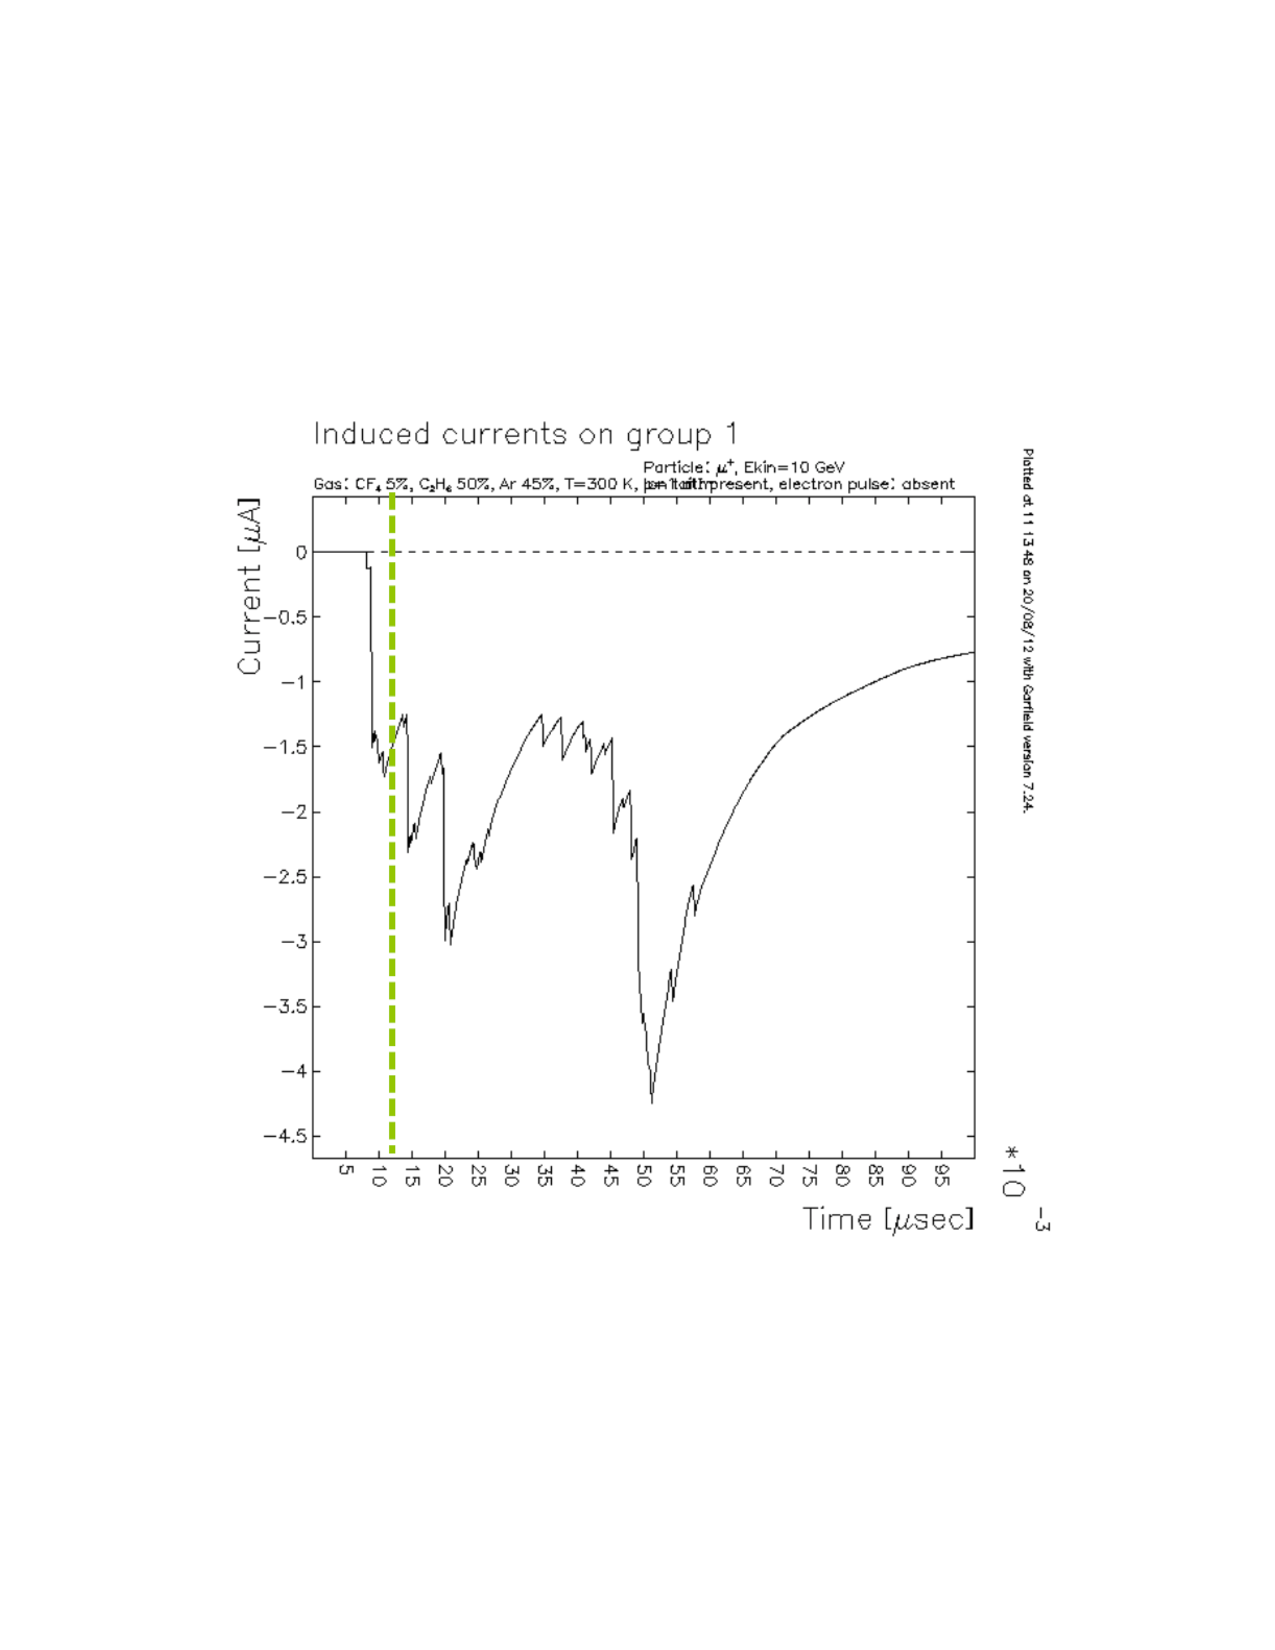
\includegraphics[width=0.55\textwidth, trim=3cm 6cm 3cm 6cm, clip]
                  {currentVtimeFifthElec}
  \caption{Garfield simulation of the induced signal current versus the arrival
    time.  The green line corresponds to the arrival time of the fifth election.
    This image is taken from~\cite{ran_bi}.}
  \label{fig::currentVtimeFifthElec}
\end{figure}

Two prototypes were built to gain hands on building expertise in preparation for
construction.  Both of these prototypes were constructed in a clean room in the
Nuclear Physics Lab (NPL) at UIUC.  Much of DC05 was built at the NPL as well.
The two prototypes were called prototype A and prototype B.  Prototype A,
Fig.~\ref{fig::protoTypeA}, consisted of 1 plane, eight sense wires, 9 field
wires and was 50~cm in length.  Prototype B on the other hand consisted of two
planes with 16 sense wires per plane and a length of 163~cm.  Prototype A was
tested with beam at DESY and was shown to achieve 200~$\mu$m
resolution~\cite{choi}.  Both of these prototypes were built using similar
materials and construction techniques as the full size detector.  In particular
these two prototypes were the needed experience for working with sense wires
having a diameter of 20~$\mu$m.

\begin{figure}[h!t]
  \centering 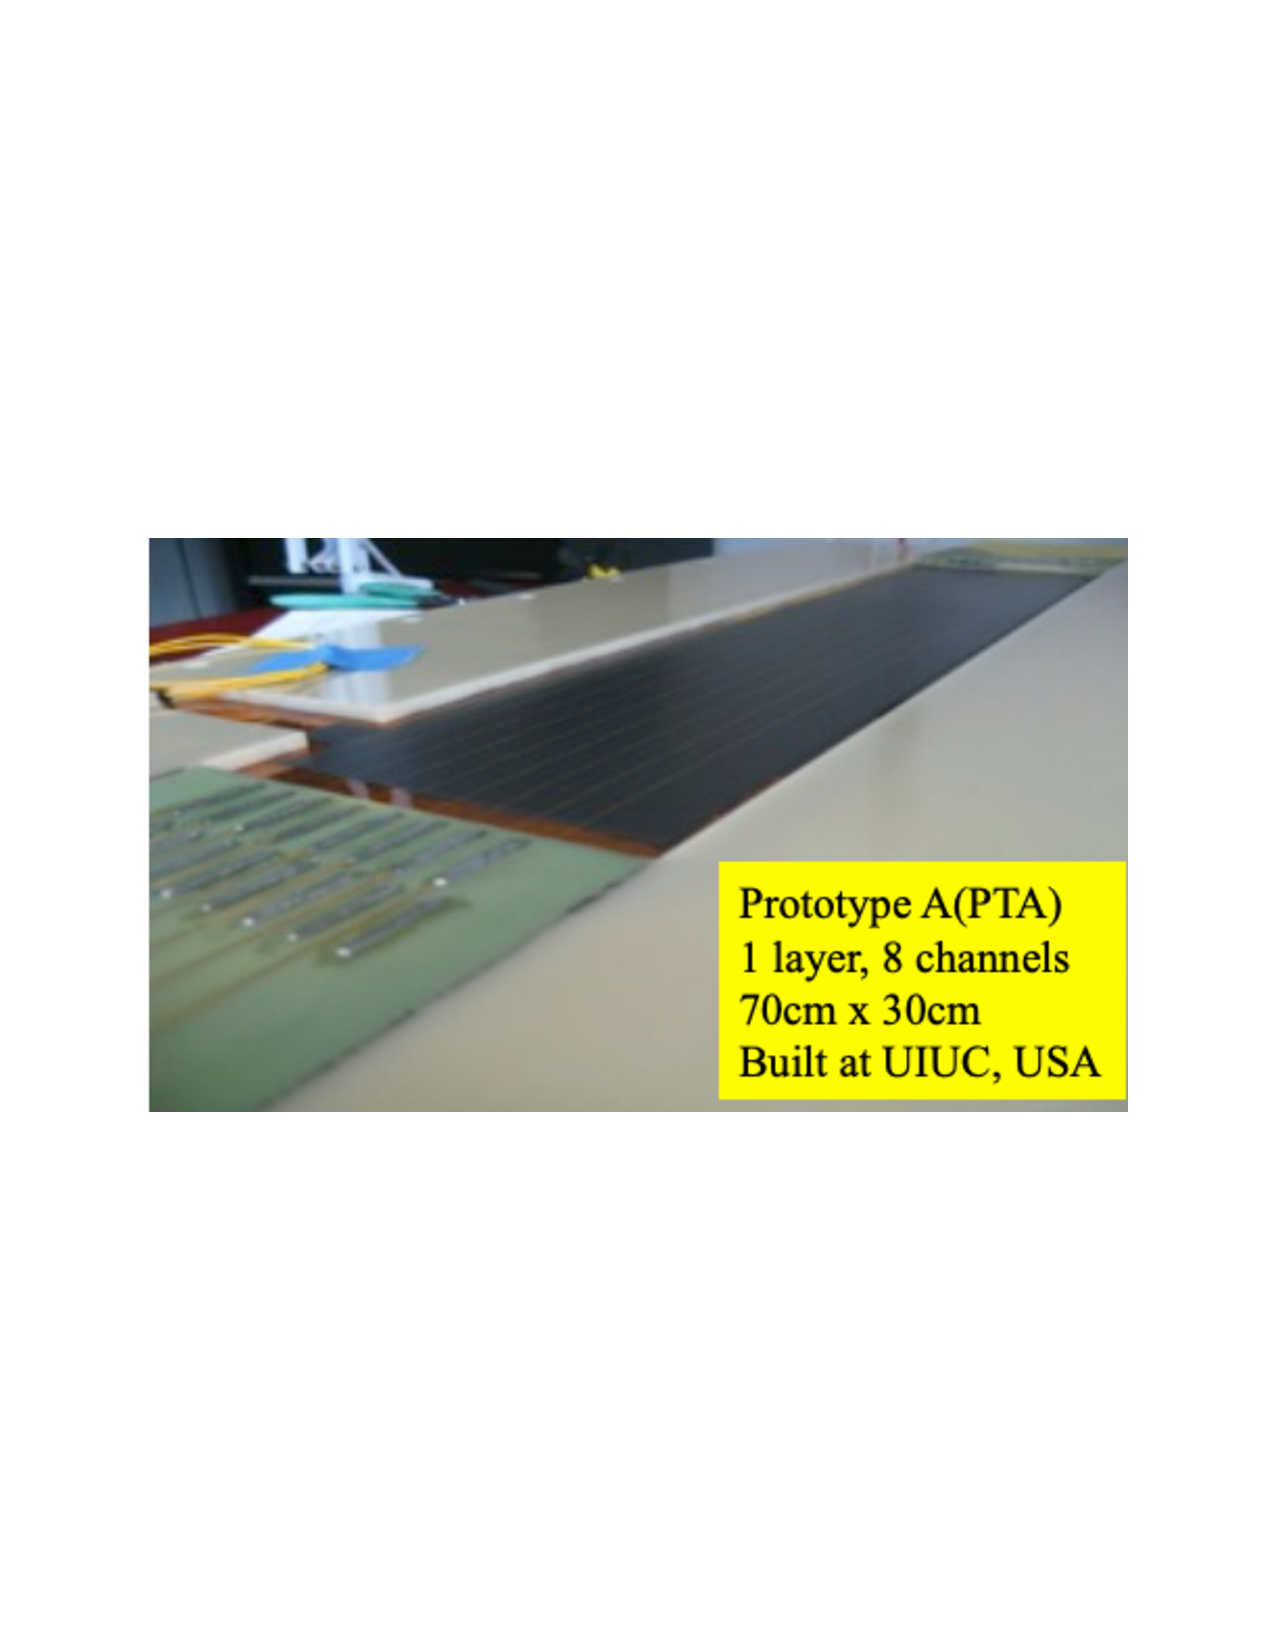
\includegraphics[width=0.6\textwidth, trim=2.5cm 8cm 2.5cm 8cm,
    clip]{protoTypeA}
  \caption{Inside view of prototype A.  This image was taken from~\cite{choi}. }
  \label{fig::protoTypeA}
\end{figure}


\section{Design}

\begin{figure}
  \centering 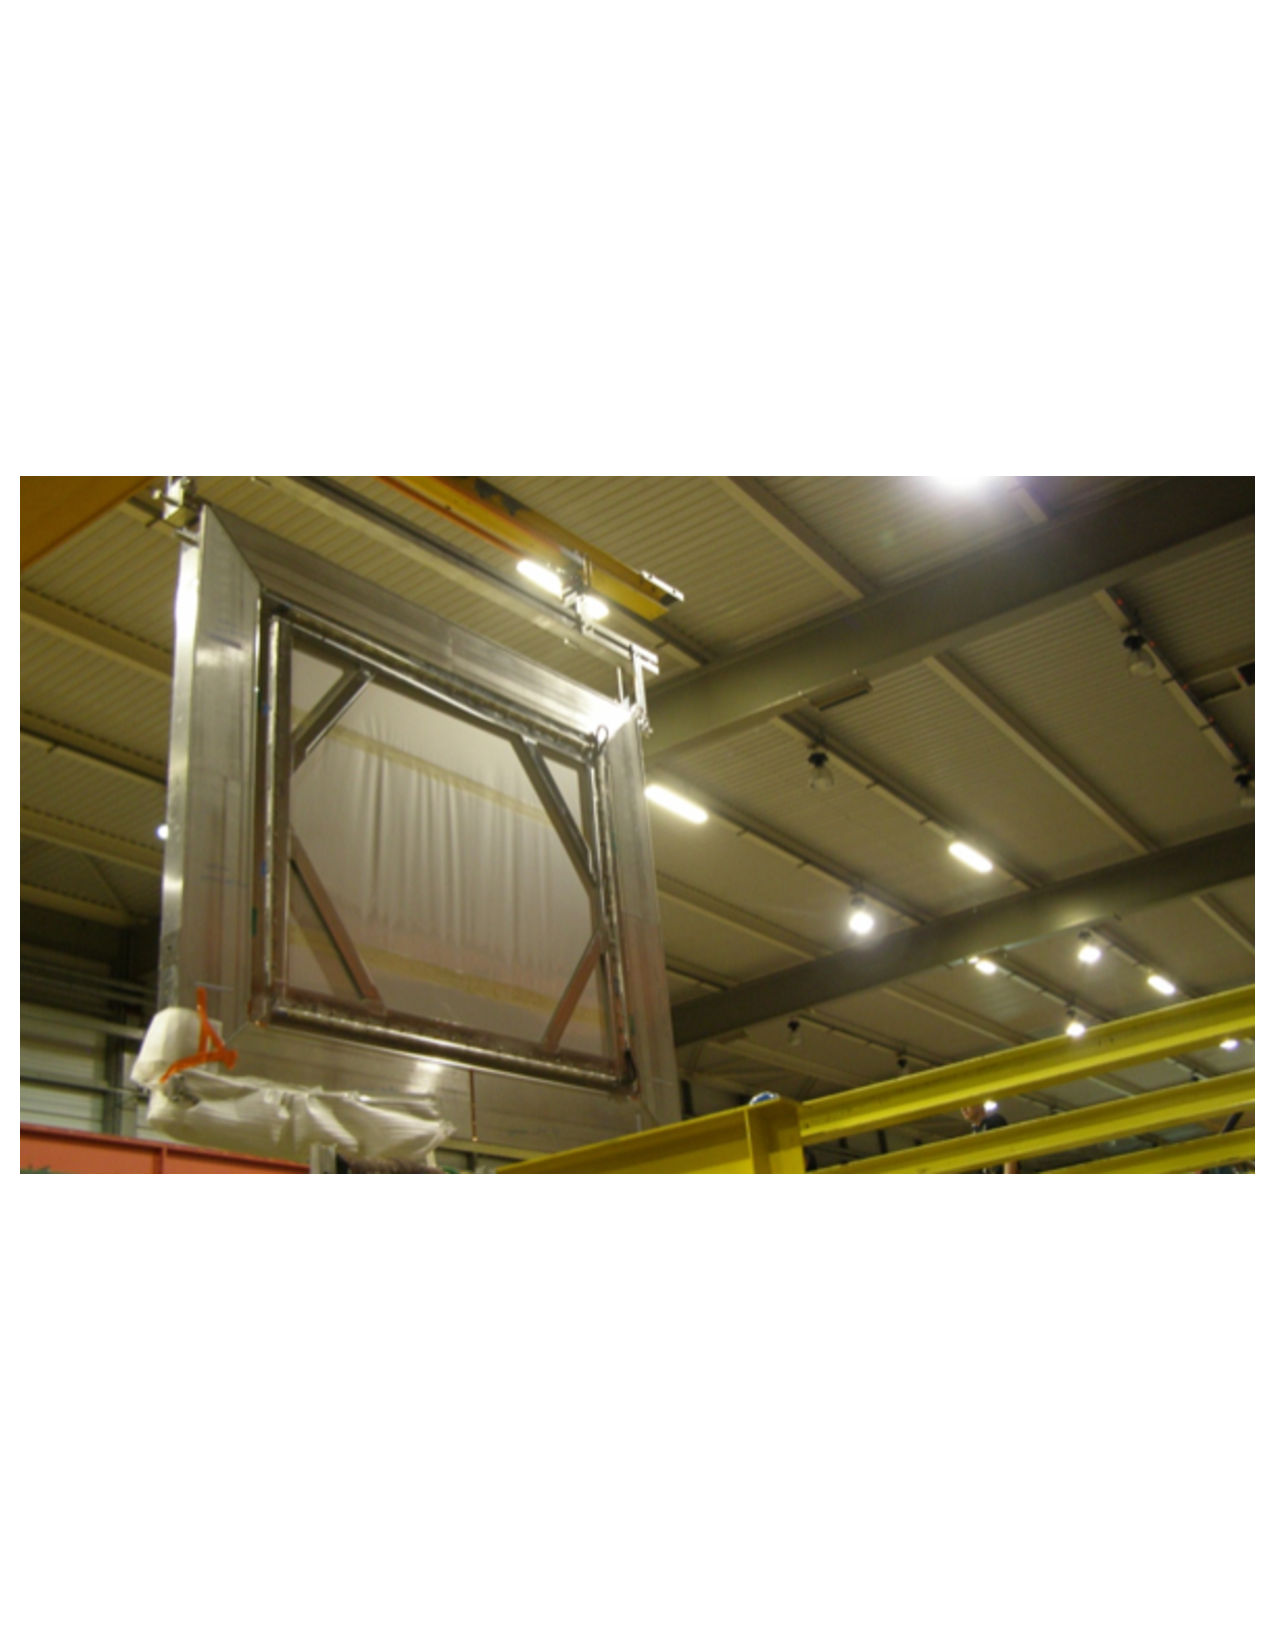
\includegraphics[width=0.7\textwidth, trim=2.5cm 8cm 2.5cm 8cm,
    clip]{DC05_full}
  \caption{}{The completed DC05 being craned into the COMPASS large area
    spectrometer.}
  \label{fig:DC05}%
\end{figure}

The design of DC05, figure~\ref{fig:DC05}, was based off a previous large-area
tracker at COMPASS.  DC05 has an active area of 249x209cm$^2$ and consists of
eight detector planes.  The eight planes of DC05 correspond to four views, where
each view measures a coordinate.  The coordinates measured from DC05 are the
horizontal, vertical and $\pm$ 10$^{\circ}$ with respect to the horizontal.  The
horizontal and vertical coordinates consist of 2x256 sense wires and the offset
to horizontal coordinates each consist of 2x320 wires for increased acceptance.
In total DC05 includes 2304 sense wires and 2312 field wires.  Each plane was
made from a G-10 frame and five frames stacked together constituting a view.
The whole detector was closed in with two precision, stainless steel stiffening
frames, which were assembled with aluminized mylar as a gas window.  The gas
window served the double purpose of holding in all the gas and electrically
isolating the sense and field wires.

The views of DC05 consist of three cathode layers and two anode layers.  The
cathodes layers were made from carbon paint sprayed on a 25~$\mu$m thin mylar
layer.  There were two single-layer cathodes layers and one layer with carbon on
two sides within each view.  Fig.~\ref{fig::DC05_layers} shows a side view of
the layers of DC05.  Additionally a 30~cm circular so-called beam killer was
added to the cathodes to control the efficiency in the central part of the
detector.  The cathodes were nominally set to -1675~V and the beam killer
voltage was set to -900~V for zero efficiency in the high flux central region.
The voltage on the beam killer can however be raised above the amplification
threshold if the beam flux is reduced and it is desirable to study the central
region.

\begin{figure}[h!t]
  \centering 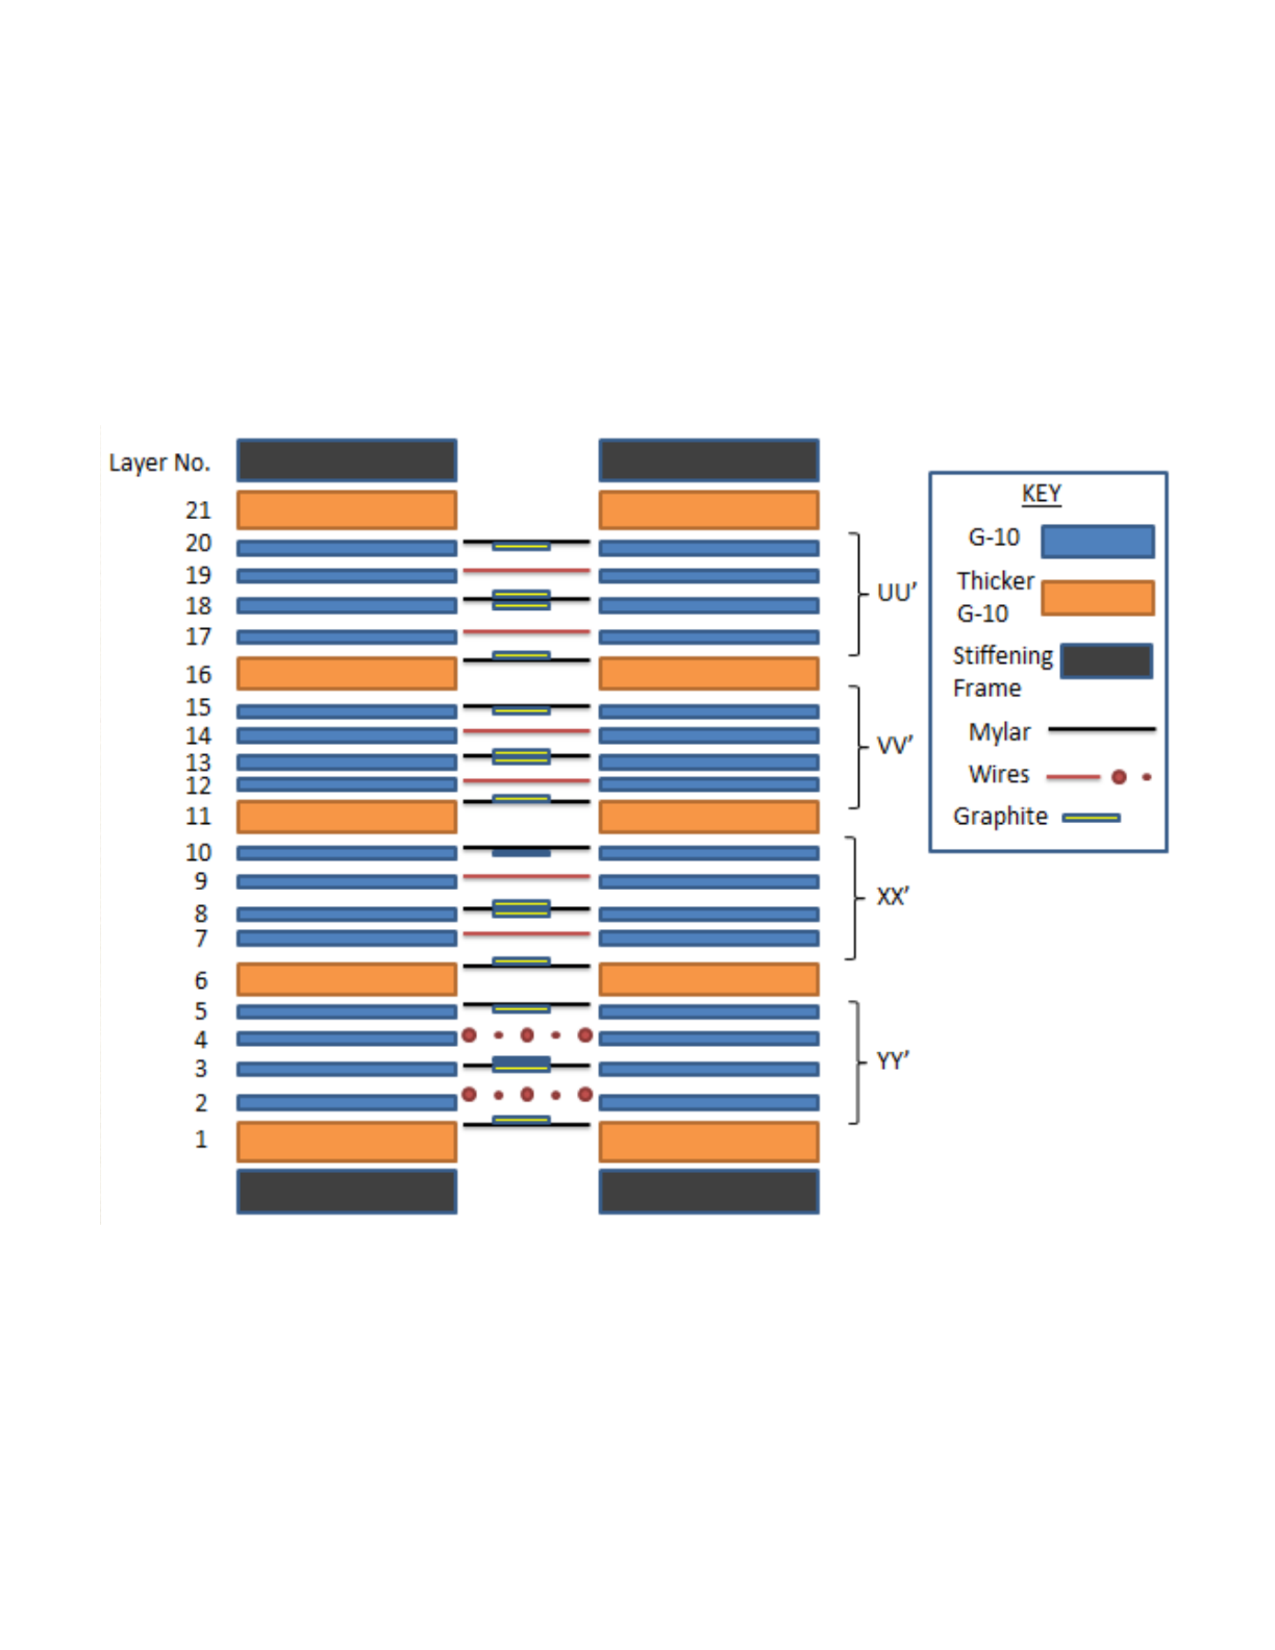
\includegraphics[width=0.7\textwidth, trim=0.2cm 7cm 0.2cm 2cm,
    clip]{DC05_layers}
  \caption{A side view sketch of the layers in DC05.  This image taken
    from~\cite{heitzDC05DNP}.}
  \label{fig::DC05_layers}
\end{figure}

The anode layers were made from alternating 20~$\mu$m gold-plated tungsten sense
wires and 100~$\mu$m gold-plated copper beryllium field wires, as depicted in
figure~\ref{fig:driftcell}.  Gold plating was used for both sense and field
wires to prevent aging effects.  The field wires were also placed at -1675~V and
the sense wires were at 0~V.  The nominal gain of DC05 is approximately 10$^4$.

\begin{figure}
  \centering 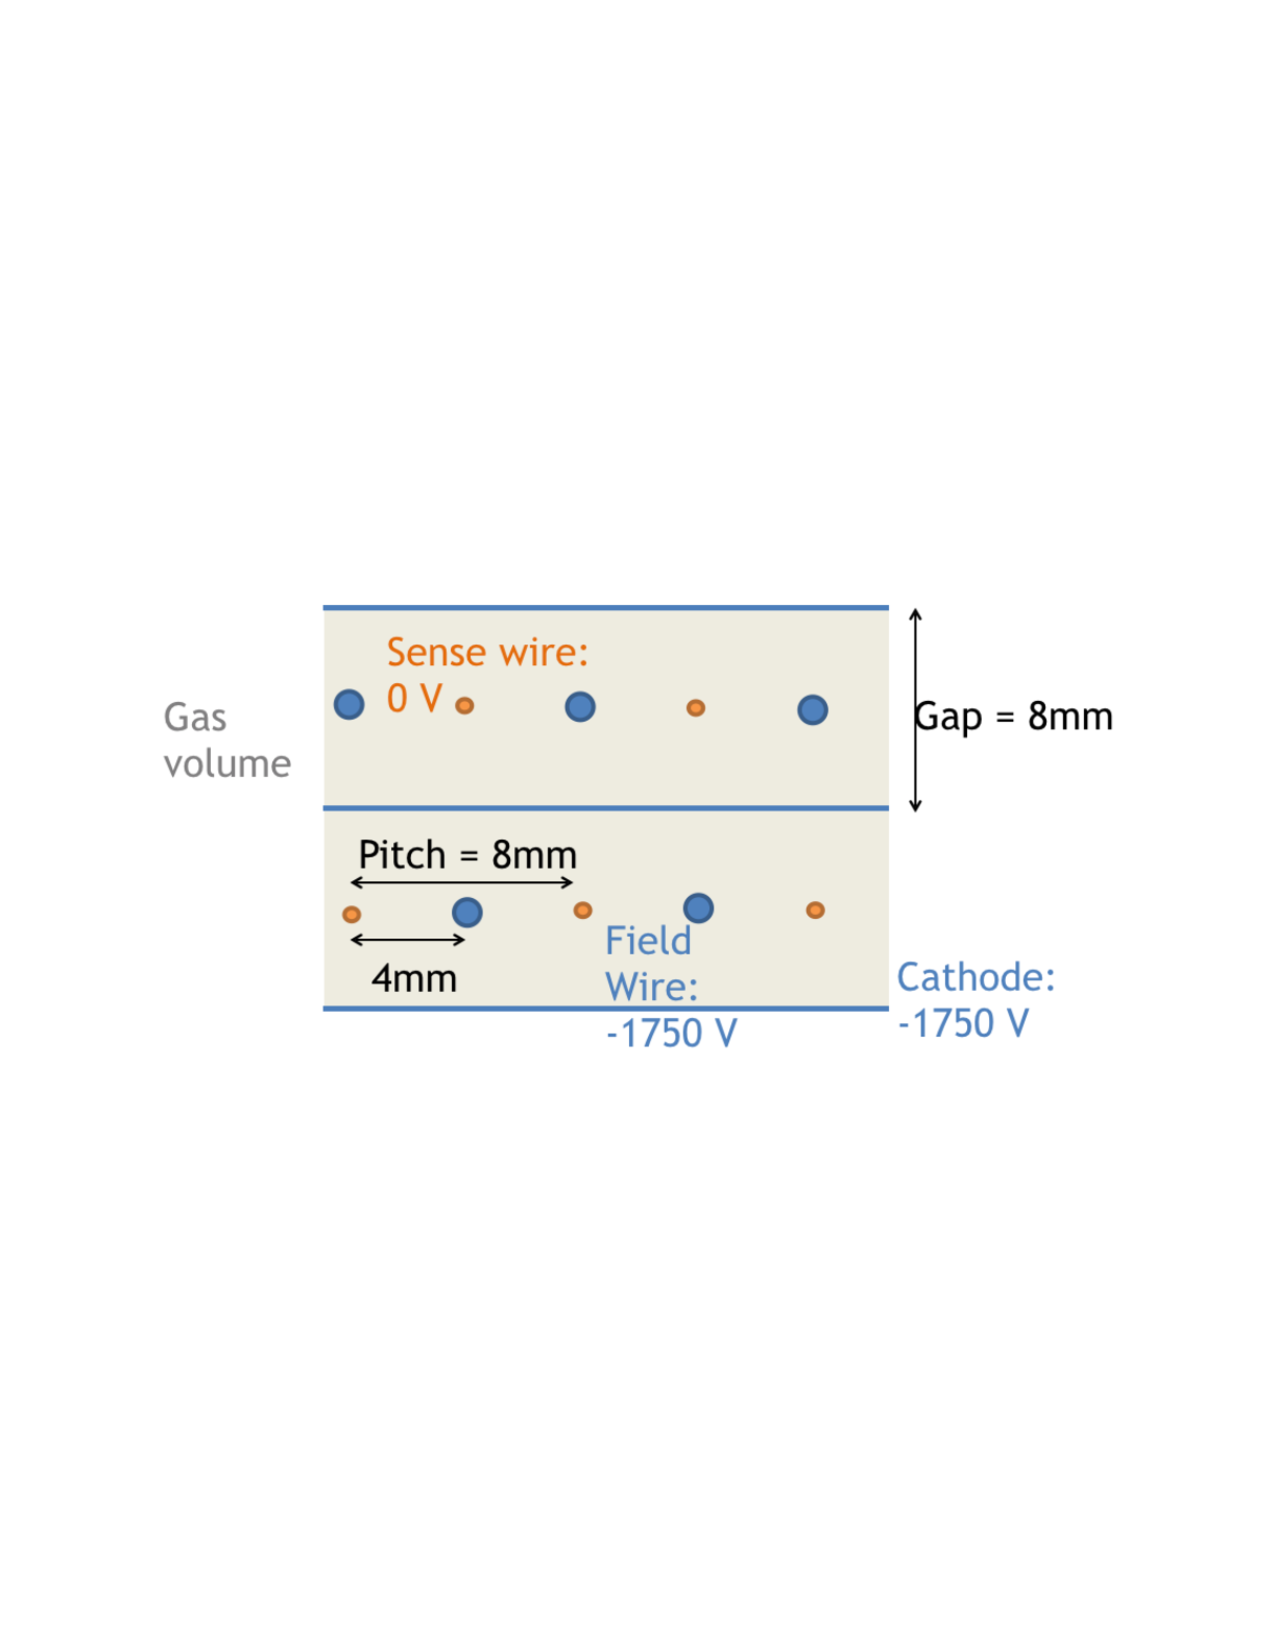
\includegraphics[width=0.5\textwidth, trim=2.5cm 10cm 3cm 10cm,
    clip]{DriftCell}
  \caption{}{The drift cell dimensions of one plane in DC05.  This image taken
    from~\cite{heitzDC05DNP}.}
  \label{fig:driftcell}%
\end{figure}

During data taking, DC05 is filled with a mixture 45\% argon, 45\% ethane and
10\% CF$_4$.  The noble gas, argon, is the gas that is ionized and amplified,
while ethane is used as a quencher and CF$_4$ is used to reduce aging effects.
The quencher, ethane, absorbs photons from the electron avalanche which could
pair produce and therefore make more electrons which would distort the electric
field in a drift cell.  The quencher therefore is used to reduce the avalanche
and ensure the drift cell electric field lines are closer to their design
values.


\section{Construction}

The construction of DC05 was carried out as precisely as possible starting with
the precision from the stainless steel stiffening frames.  The overall flatness
of the detector was designed to be flat within +50~$\mu$m -0$\mu$m.  To achieve
this the stiffening frames where cut with the highest relative accuracy by
cutting the two frames on top of each other to a precision of 50~$\mu$m
everywhere in their plane.  The precision from the stiffening frames was
transferred to the anode and cathode frames through 40 positioning pins.  The
G-10 frames were milled from strips at the NPL using a precision milling
machine.  Each four strips were then epoxied together on top of one of the
stiffening frames to best transfer the precision of the stiffening frame.

The Atlas Tool and Die Works company machined the stiffening frames out of
stainless steel.  It was very import to construct the detector from stainless
steel as DC05 resides in a strong fringe field from the first spectrometer
magnet.  The gluing procedure was carried out in teams at the NPL.  The epoxy
used was STYCAST 1266 which is a two component and has low viscosity.  The epoxy
was applied to both G-10 frames glued together at a lap joint and allowed to dry
for 24 hours.  The PCB boards were similarly epoxied to the G-10 frames.

The cathodes had mylar stretched and epoxied to them using a custom built
stretching machine at CERN.  Fig.~\ref{fig::mylarStretching} shows the process
of stretching mylar on a cathode.  An external Swiss company then spray painted
carbon on them which was then polished till the resistance was approximately
30~k$\Omega /m$.  All the sense and field wires were hand soldered as shown in
Fig.~\ref{fig::wireSoldering}, and sequentially verified for position using a
microscope.  It was estimated the position placement of each sense wire was at
least as good as half the diameter of a sense wire or precise to 10~$\mu$m.

\begin{figure}[h!t]
  \centering 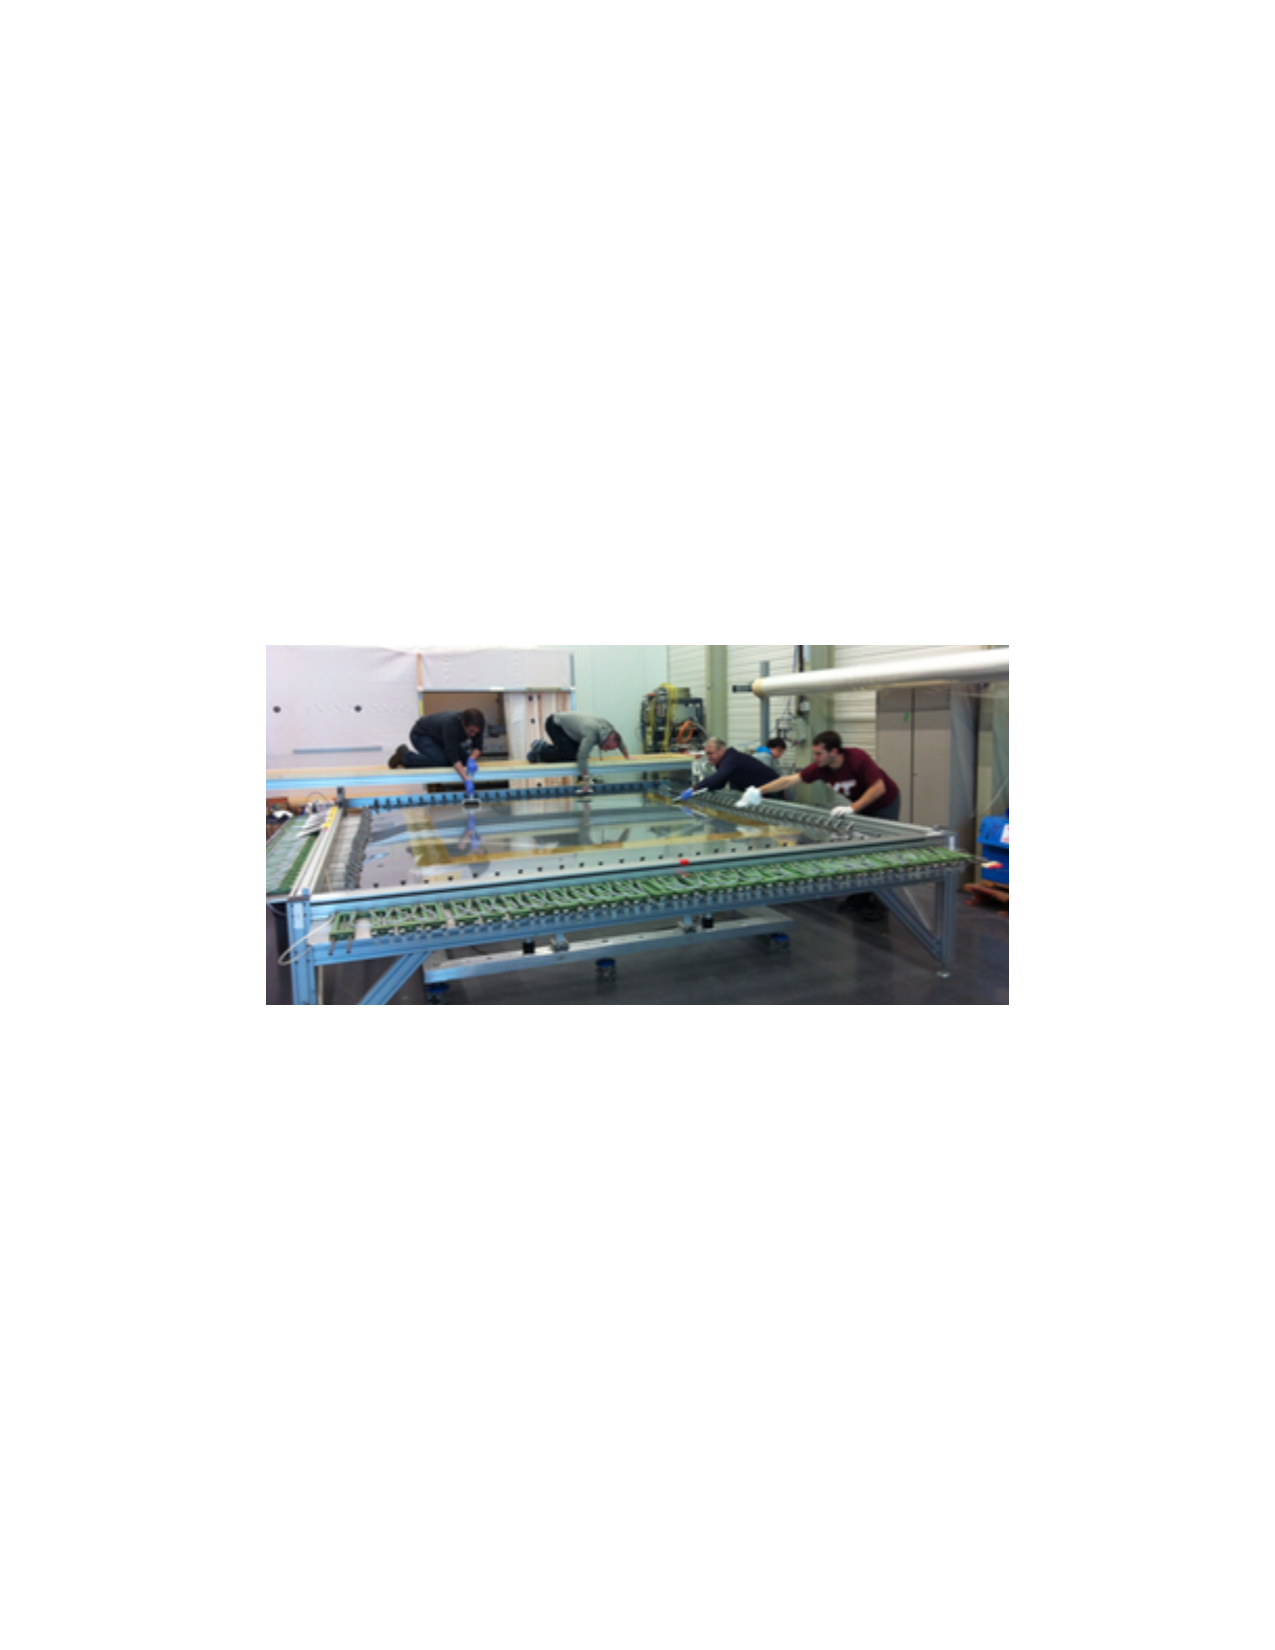
\includegraphics[width=0.6\textwidth, trim=5cm 12cm 5cm 10cm,
    clip]{mylarStretching}
  \caption{Stretching mylar on a cathode plane at CERN}
  \label{fig::mylarStretching}
\end{figure}

\begin{figure}[h!t]
  \centering 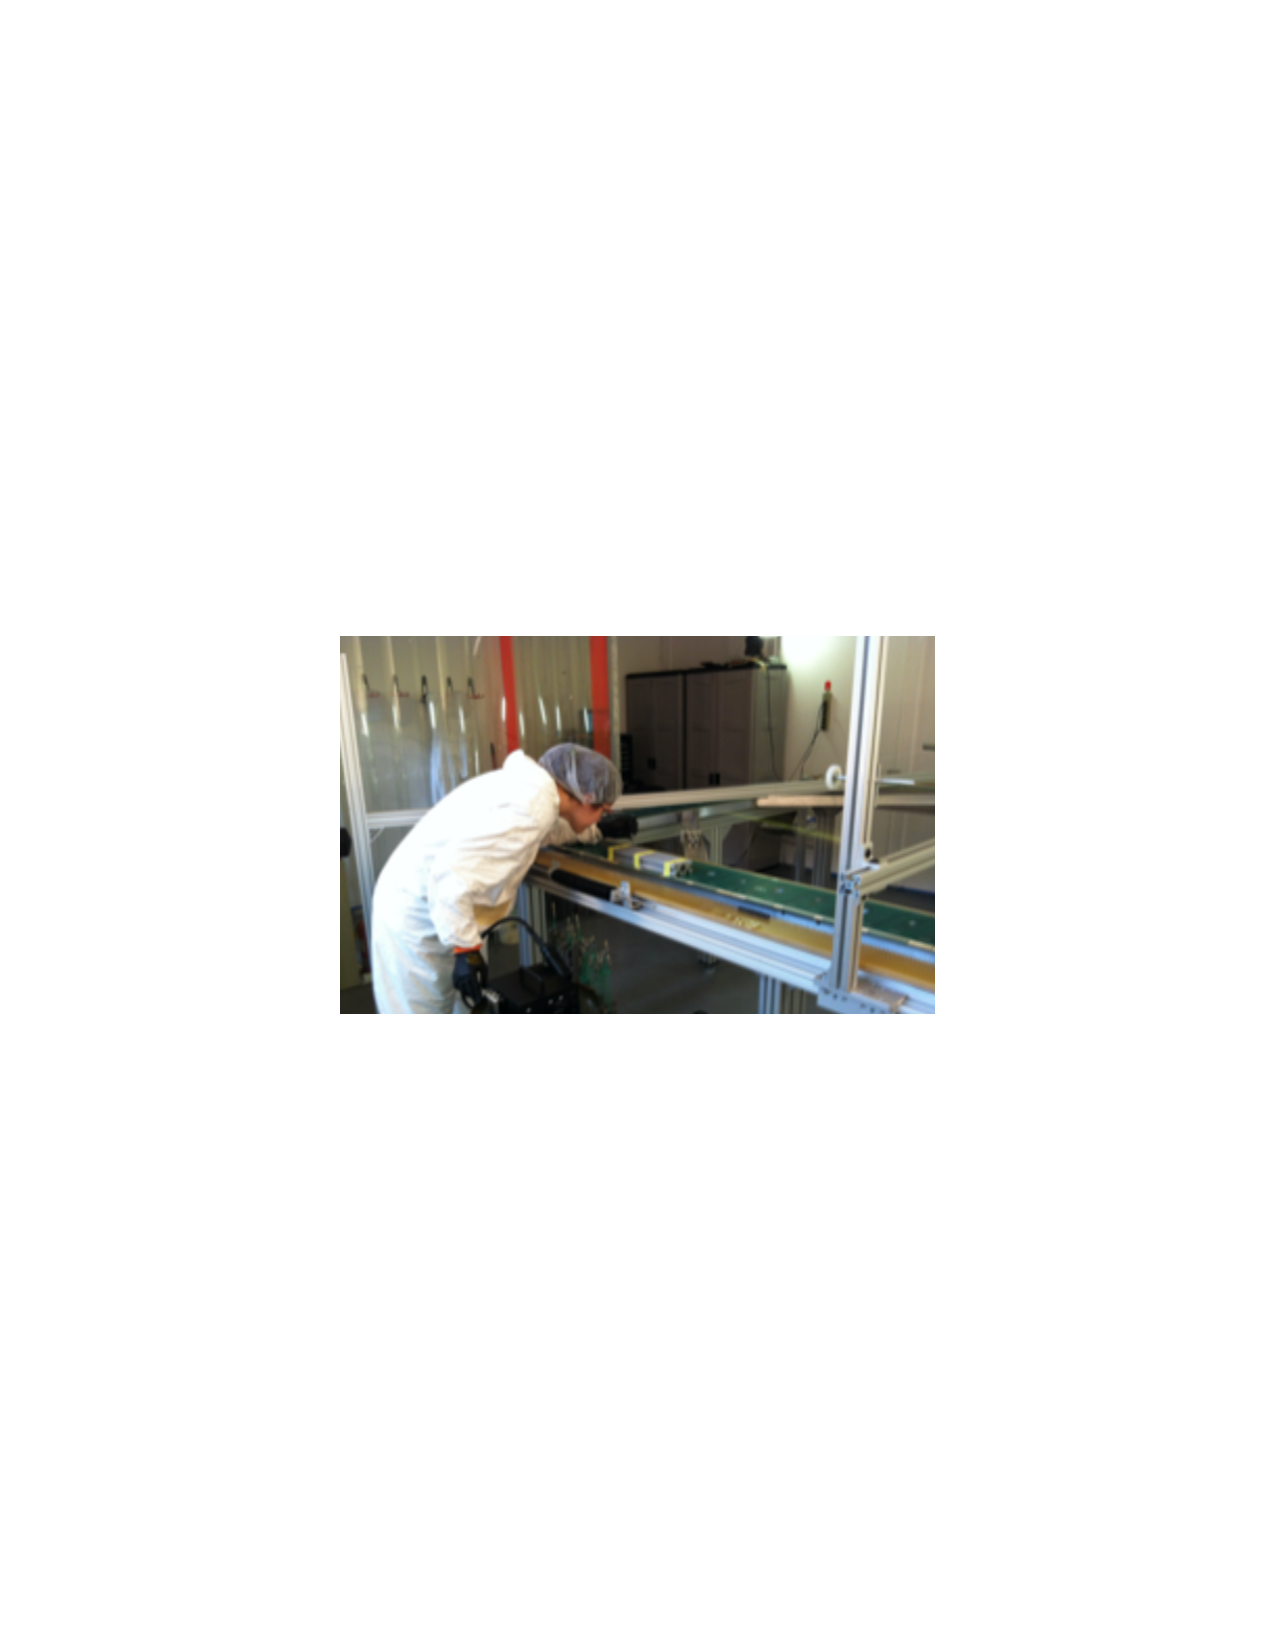
\includegraphics[width=0.6\textwidth, trim=5cm 10cm 5cm 10cm,
    clip]{wireSoldering}
  \caption{Hand soldering DC05 wires in the clean room at the NPL}
  \label{fig::wireSoldering}
\end{figure}

The final assemble was done at CERN.  This consisted of stacking each of the 21
G-10 frames on top of the stiffening frame, Fig.~\ref{fig::cernFinalAssembly},
and attaching copper electronic shielding all along the exterior of the detector
to reduce electronic noise.

\begin{figure}[h!t]
  \centering 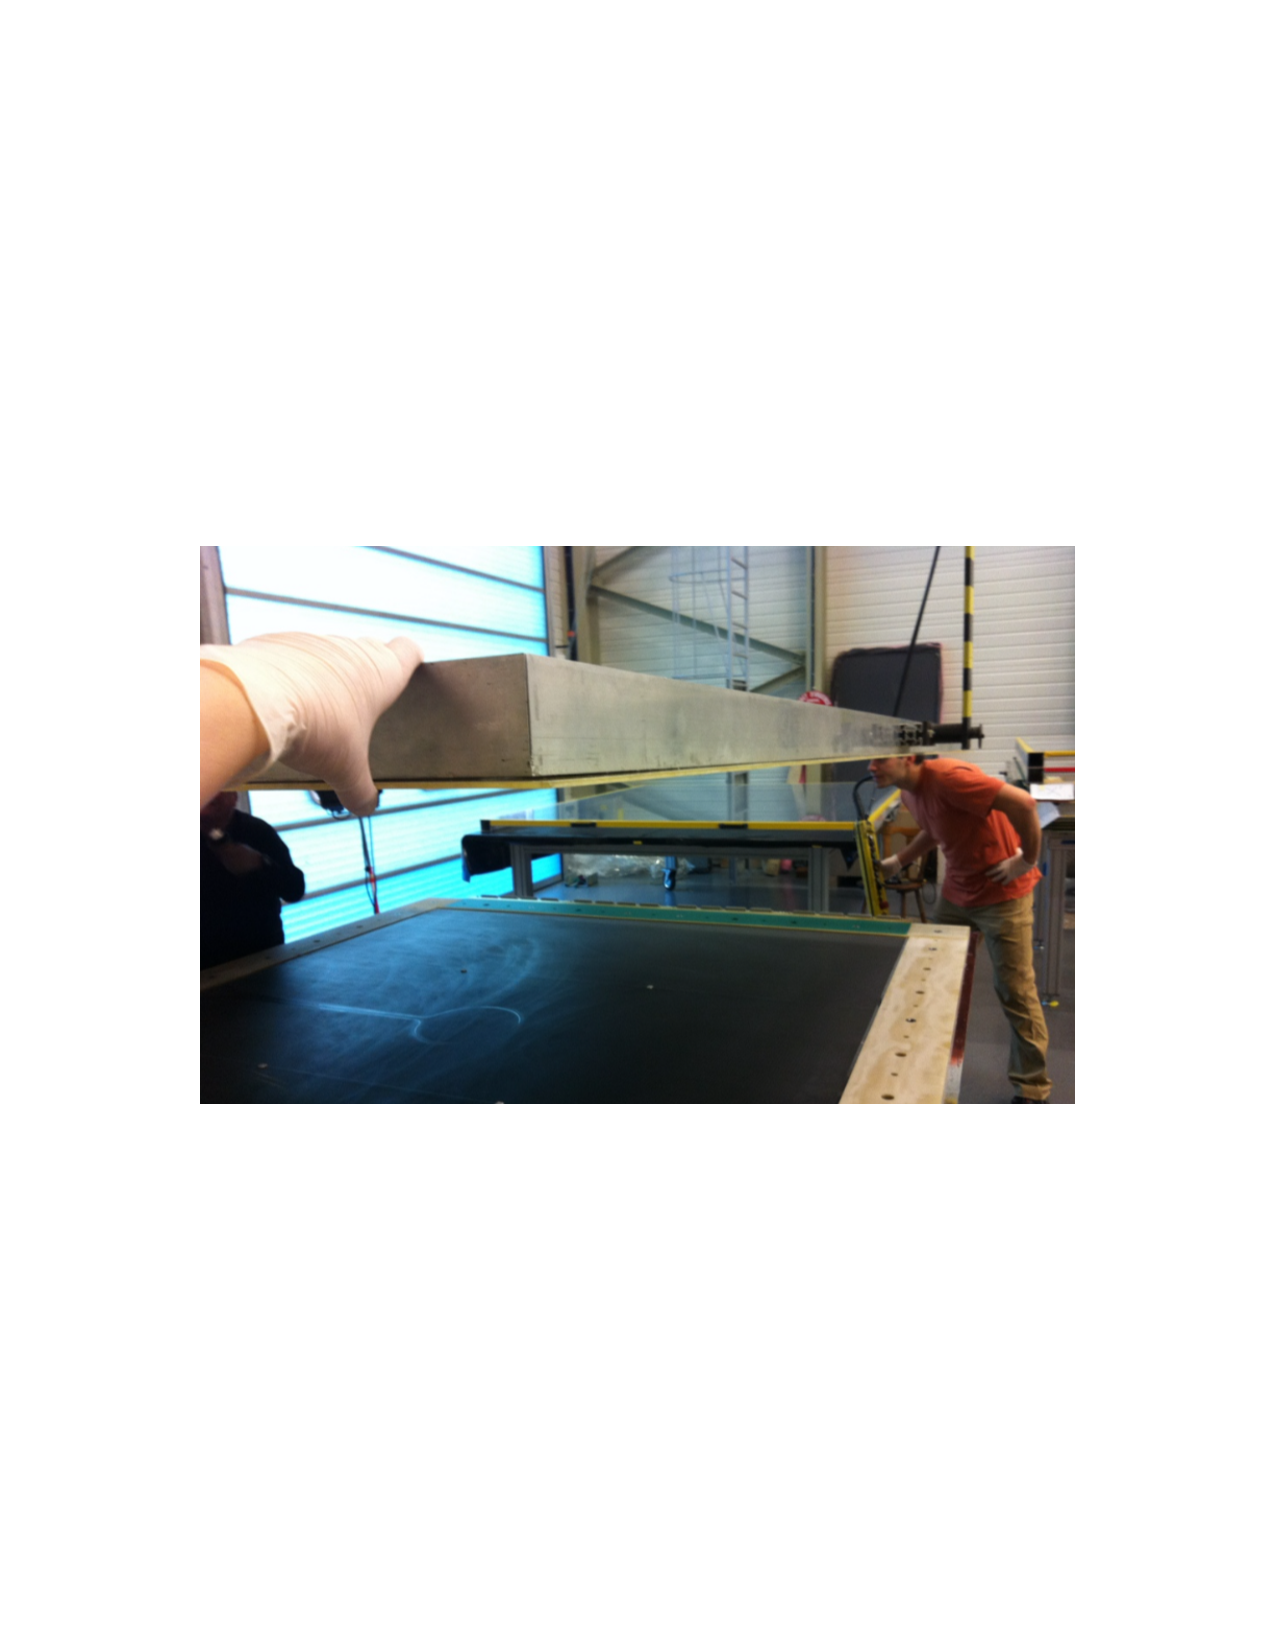
\includegraphics[width=0.6\textwidth, trim=5cm 10cm 5cm 10cm,
    clip]{cernFinalAssembly}
  \caption{The process of stacking the G-10 frames at CERN}
  \label{fig::cernFinalAssembly}
\end{figure}

There were various tests performed throughout the construction process for
quality assurance before the final installation.  The starting tests were
measuring thickness and position of important cuts on the G-10 strips using a
micrometer.  G-10 strip thicknesses were iteratively milled until they reached
better than 50~$\mu$m in thickness accuracy.  The thickness deviation of the
whole detector including the stainless steel stiffening frames was better than
750~$\mu$m.  The mechanical tension of the sense wires was tested for stability
by ensuring the voltage difference between sense and field wires could reach as
high as 2400~V in air.  In addition the wire tension was cross-checked by
determining the resonance frequency with which the wires vibrated.  The
resonance frequency was determined by placing the wires in a constant magnetic
field and varying a sinusoidal current across each wire till the wires vibrated
maximally.  The leakage current between sense and field wires was verified to be
less than 100~nA at nominal voltage in air.  Finally amplification tests were
first performed using a strontium-90 source and verifying the counts per
electronics board increased below the radioactive source.


\section{2015 Performance}

The overall performance of DC05 was checked using the COMPASS reconstruction
software CORAL (discussed in sec~\ref{sec::dataReconstruction}).  In all cases
the view of study was excluded from the reconstruction algorithm and the
individual hit information for the view of interest was saved to get an unbiased
measurement.  The performance of DC05 is determined by judging its response to
real tracks.  In other words tracks that are not falsely reconstructed,
so-called ghost tracks.  To ensure these real tracks with higher quality for
performance evaluation, only tracks with a primary vertex near the polarized
target are considered.

The efficiency was found to be between 85\% and 90\% depending on the plane.
The efficiency was determined by searching for a hit in the DC05 plane of
interest within a road of 1.2~mm from the reconstructed track location.  The
road distance was chosen to be approximately six resolution deviations which is
standard at COMPASS.  Fig.~\ref{fig::DC05Yeff} shows the efficiency of one plane
of DC05.  Using the so called RT relation, figure~\ref{fig:RT_DC05Y2}, the
location of a track within a drift cell can be most accurately determined.  This
RT relation is tuned as a calibration to minimize the track residuals.  The RT
relation also varies depending on the beam type, intensity and the trigger type.

\begin{figure}[h!t]
  \centering 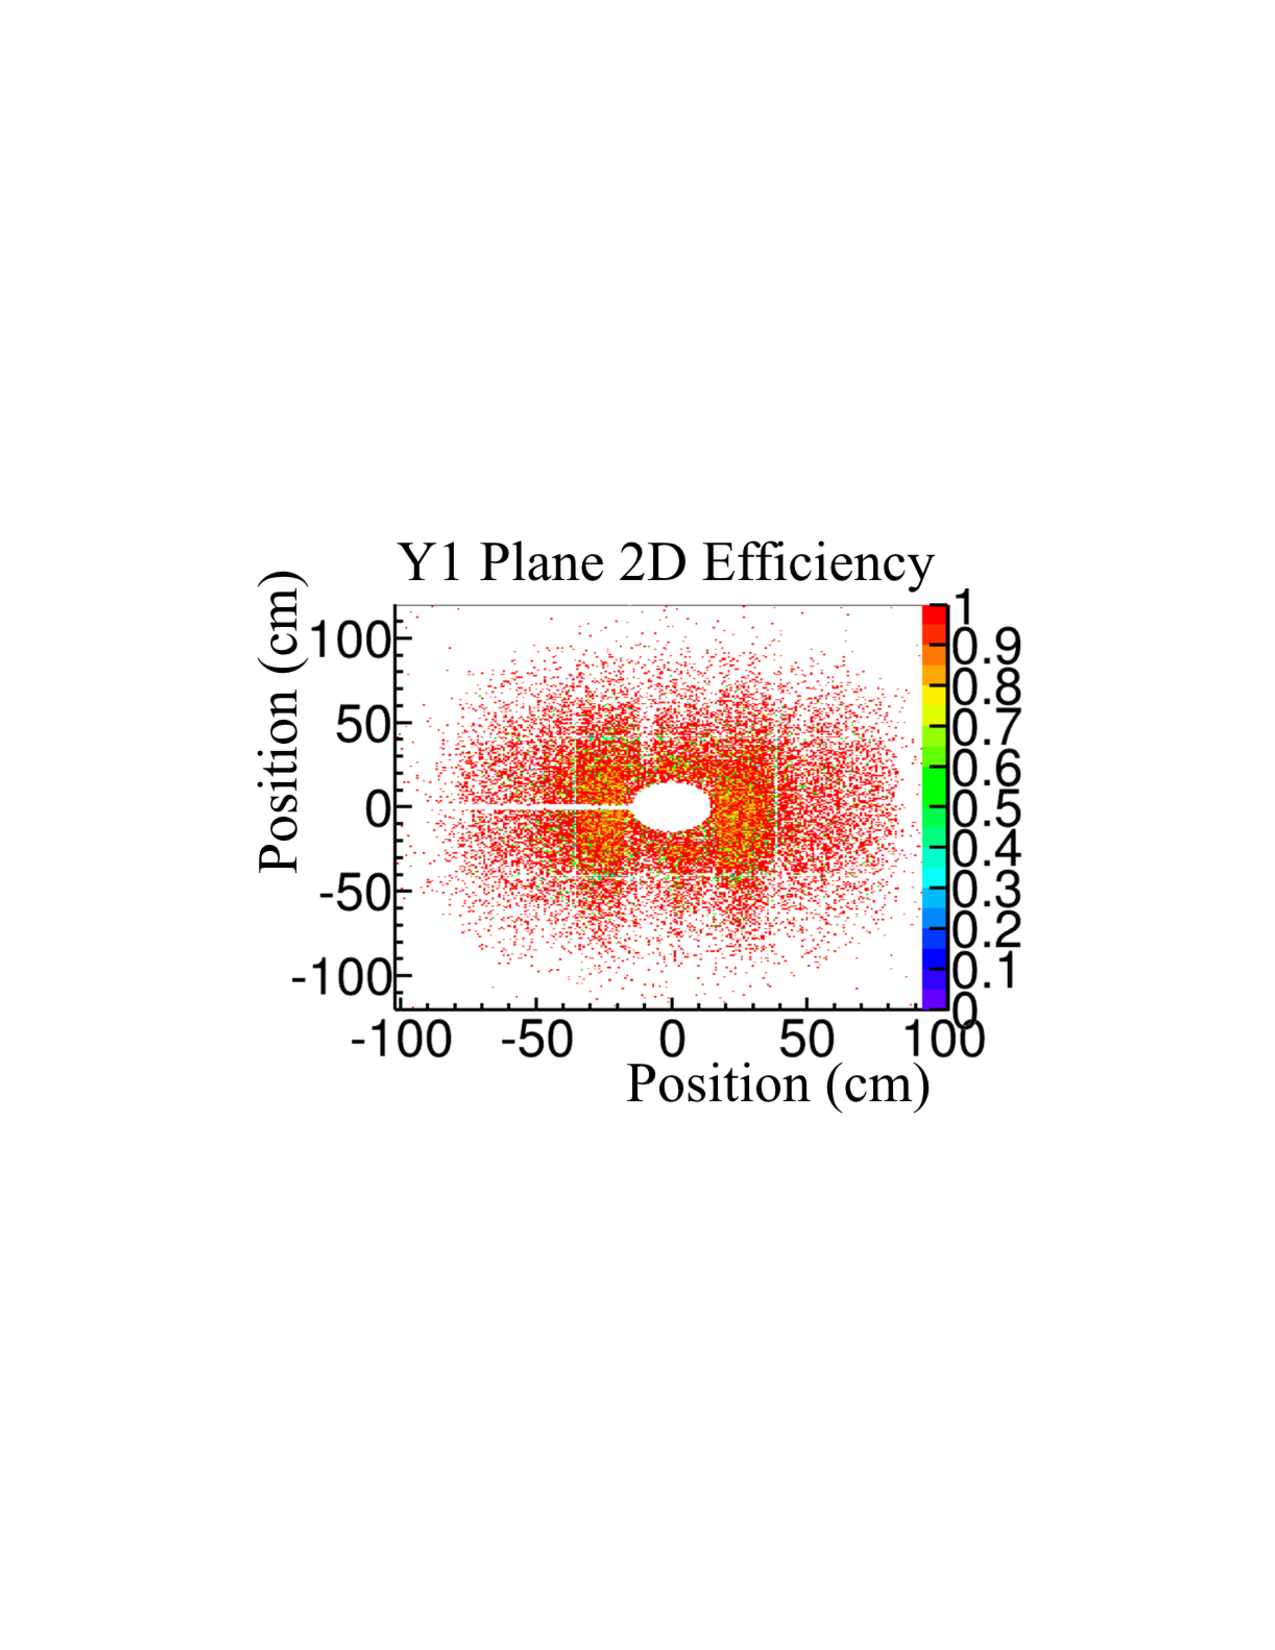
\includegraphics[width=0.6\textwidth, trim=3cm 9cm 3cm 9cm,
    clip]{DC05Yeff}
  \caption{}{Two dimensional efficiency on the DC05Y1 plane.  The center region
    with zero efficiency is a result of the beam killer.  This image taken
    from~\cite{heitzDC05Spin}.}
  \label{fig::DC05Yeff}%
\end{figure}

\begin{figure}[h!t]
  \centering 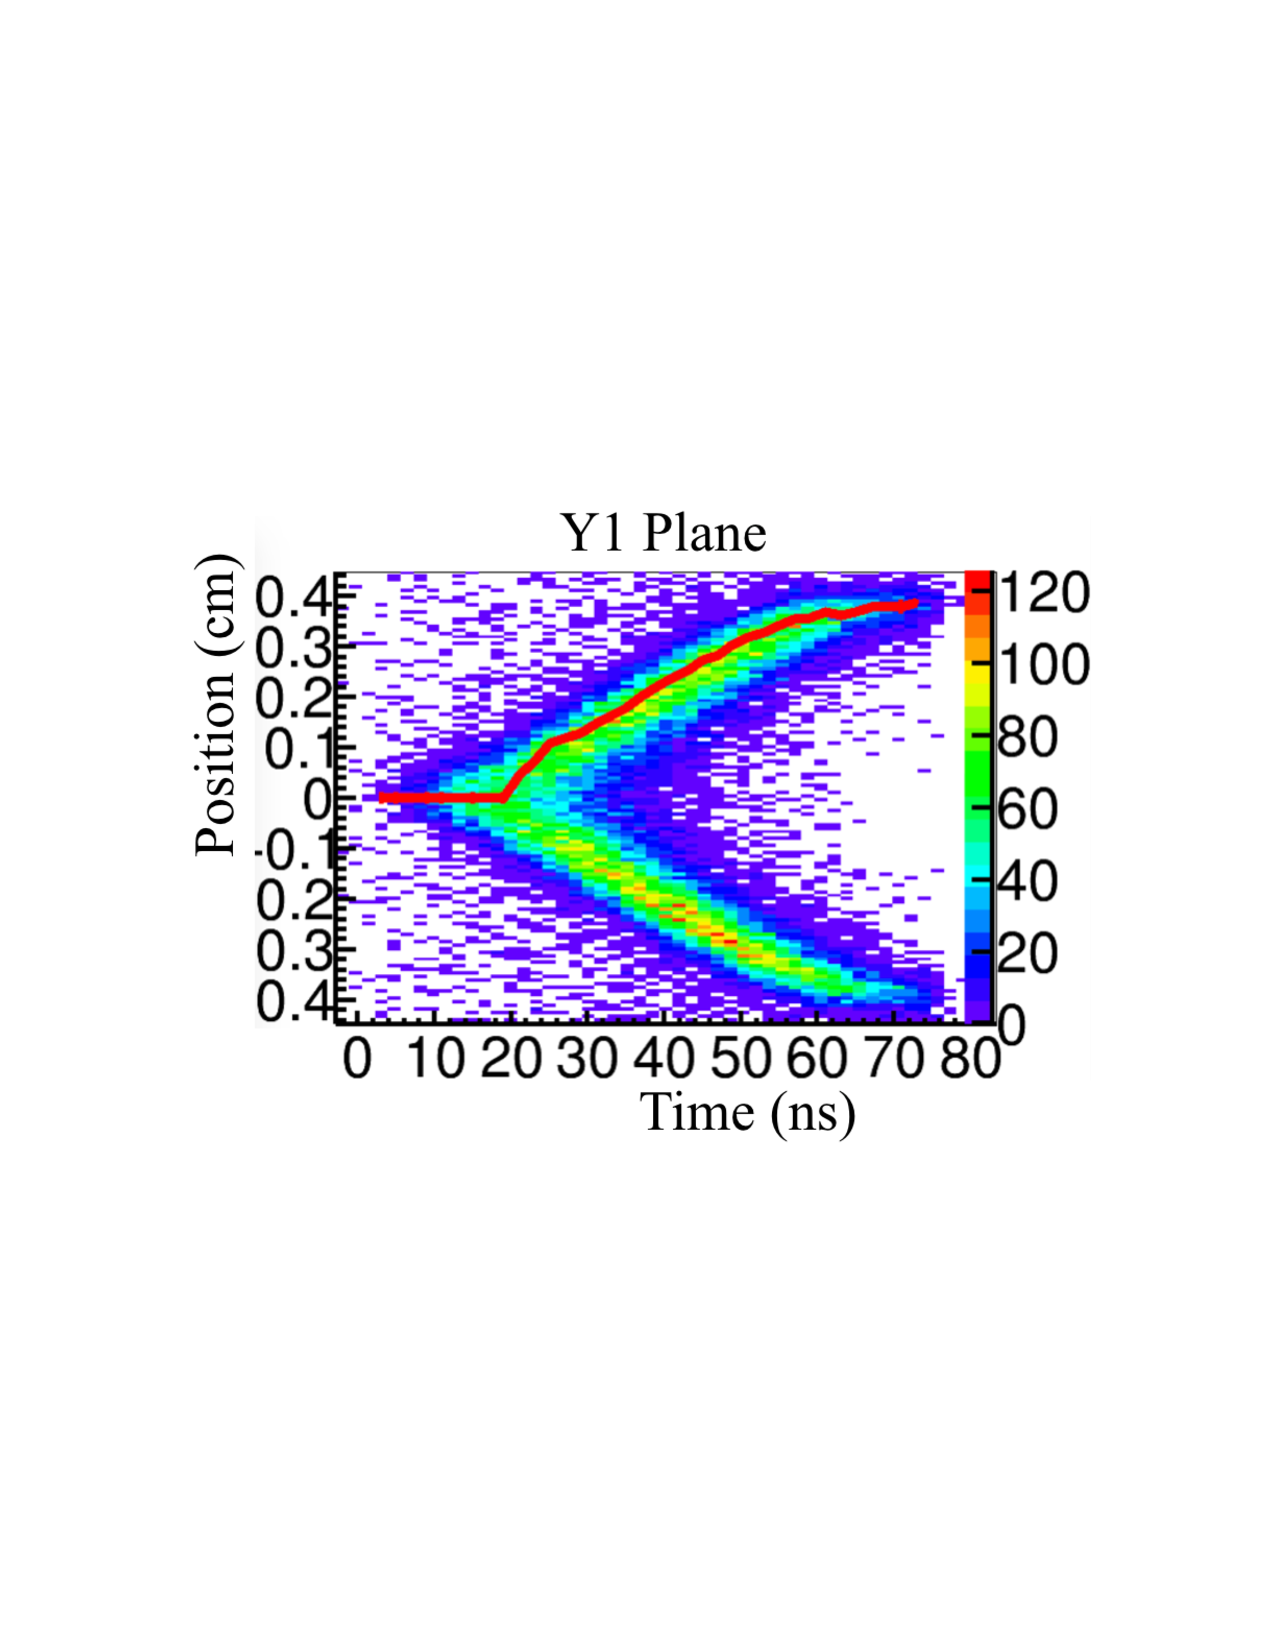
\includegraphics[width=0.6\textwidth, trim=3cm 8cm 3cm 8cm,
    clip]{RT_DC05Y2}
  \caption{}{Time versus position relation, or RT relation, after calibrating.
    The red fit shows the calibration determined.  This image taken
    from~\cite{heitzDC05Spin}}
  \label{fig:RT_DC05Y2}%
\end{figure}

The double layer residual was used to determine the position resolution.  The
double layer residual is the difference between the expected positions of the
two planes in a view.  The double residual is defined as

\begin{equation}
  \label{equ::doubleRes}
  \Delta \mathrm{u}_{\mathrm{double \; residual}} = (\mathrm{u}_{\mathrm{plane
      \; 1}} - \mathrm{u}_{\mathrm{track}}) - (\mathrm{u}_{\mathrm{plane \; 2}}
  - \mathrm{u}_{\mathrm{track}}) = \mathrm{u}_{\mathrm{plane \; 1}} -
  \mathrm{u}_{\mathrm{plane \; 2}},
\end{equation}
\noindent
where u$_{\mathrm{plane \; 1(2)}}$ is the hit position on plane 1(2) determined
from the detector of interested and u$_{\mathrm{track}}$ is the hit position
determined from reconstruction.  As can be seen in Eq.~\ref{equ::doubleRes}, the
double layer residual is independent of the track resolution and only depends on
the difference between detector hit positions.  As the detector was constructed
with a known difference between these two cell hit positions, the double
residual distribution is expected to be a constant value.  Therefore the
variance of the double residual distribution is the addition of the variance of
the two individual planes.  That is

\begin{equation}
\sigma_{\mathrm{double \; residual}}^2 = \sigma_{\mathrm{plane \; 1}}^2 +
\sigma_{\mathrm{plane \; 2}}^2 = 2*\sigma_{\mathrm{plane \; 1}}^2,
\end{equation}

\noindent
where $\sigma_{\mathrm{plane \; 1(2}}$ is the position resolution of plane 1(2).
It is assumed that the position resolution is the same for each plane and
therefore

\begin{equation}
\sigma_{\mathrm{plane \; 1}} = \sigma_{\mathrm{plane \; 2}} =
\frac{\sigma_{\mathrm{double \; residual}}}{\sqrt{2}}
\end{equation}

\noindent
For the 2015 Drell-Yan physics taking the resolution achieved was approximately
430~$\mu$m. This was determined by fitting the double residual with a Gaussian
to extract the variance and assuming equal variance per plane in a view as is
shown in Fig.~\ref{fig::DC05doubleRes}.  The difference between the position
resolution for the full detector and that of the prototypes is attributed to be
due to the large area of the detector and the high beam flux in the data taking.
It is not ruled out that software improvement can be made in the future to
improve the position resolution.  One possible solution would be to include a
different RT calibration curve for each section of the detector depending on the
particle flux.

\begin{figure}[h!t]
  \centering 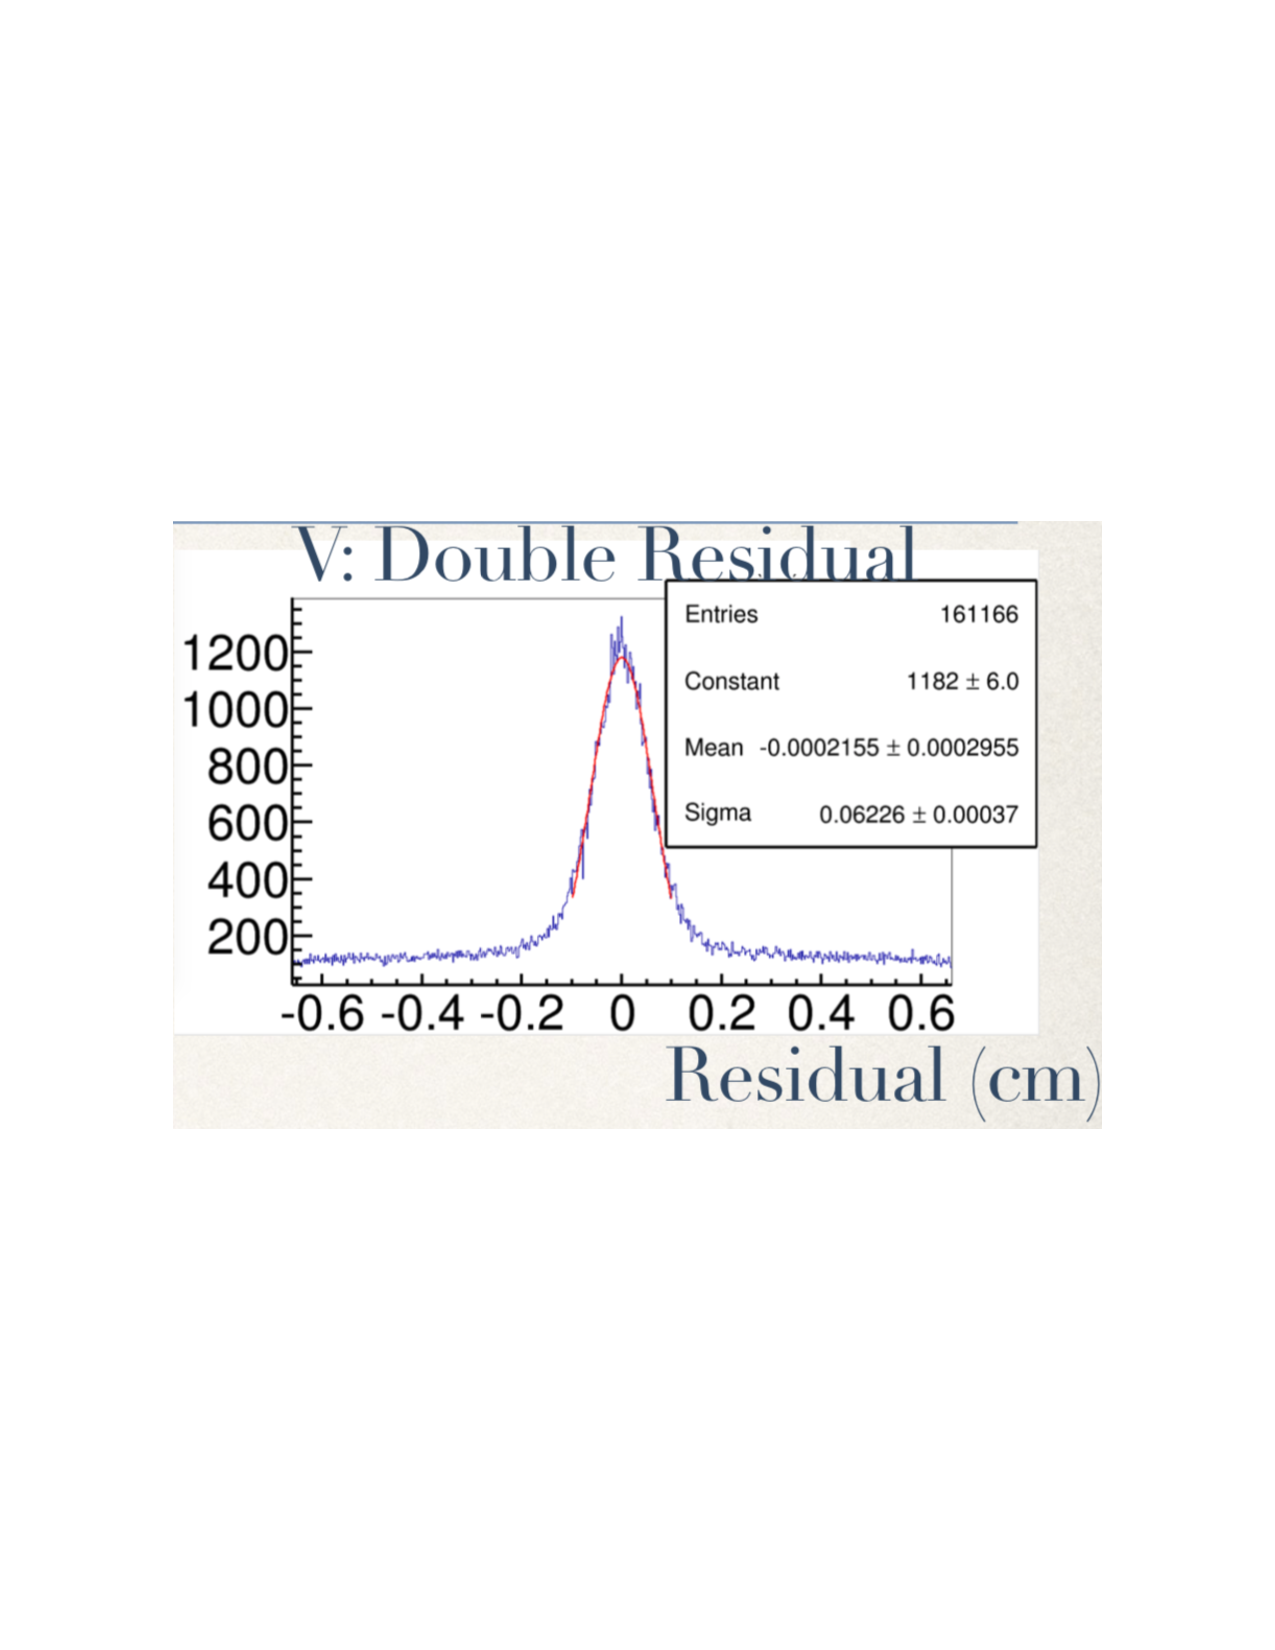
\includegraphics[width=0.6\textwidth, trim=3cm 9cm 3cm 9cm,
    clip]{DC05doubleRes}
  \caption{The double residual distribution for the U plane together with a
    Gaussian fit in red to determine the variance of the distribution.  This
    image taken from~\cite{heitzDC05Spin}.}
  \label{fig::DC05doubleRes}
\end{figure}
